\documentclass[11pt,a4paper,table]{beamer}
\mode<presentation>

\usepackage[spanish]{babel}
\usepackage[utf8]{inputenc}
\usepackage{amsmath}
\usepackage{amsfonts}
\usepackage{amssymb}
\usepackage{graphicx}

\graphicspath{{../img/}{img/}}
\usetheme[secheader]{Boadilla}
% diagramas temporales
\newcounter{wavecount}

\AtBeginSubsection[]
{
	\begin{frame}<beamer>{Agenda}
		\tableofcontents[sections=\thesection,currentsubsection]
	\end{frame}
}
\usepackage{siunitx}
\usepackage{listings}
\usepackage{tikz}
\usetikzlibrary{arrows,babel,backgrounds,fit,patterns,petri,positioning,shapes}

\tikzstyle{core}=[
	rectangle,
	rounded corners,
	draw=black,
	minimum size=40]

\tikzstyle{perif}=[
	core,
	minimum height=20]

\tikzstyle{contenedor}=[
	rectangle,
	draw=black]

\tikzstyle{exterior}=[
	rectangle,
	draw=black,
	minimum size=40]

\tikzstyle{bloque}=[
	exterior,
	align=center,
	minimum size=60,
	text width=60]

\tikzstyle{pid}=[
	draw=black,
	align=center,
	rectangle,
	rounded corners,
	minimum width=20,
	minimum height=110,
	pattern=north east lines,
	pattern color=black!35]

\tikzstyle{dir}=[
	draw,
	rectangle,
	rounded corners,
	minimum width=20,
	minimum height=110,
	align=center]

\tikzstyle{data}=[
	draw=black,
	align=center,
	rectangle,
	rounded corners,
	minimum width=120,
	minimum height=110,
	fill=black!05]

\tikzstyle{crc}=[
	draw=black,
	align=center,
	rectangle,
	rounded corners,
	minimum width=20,
	minimum height=110,
	pattern=dots,
	pattern color=black!25]

\tikzstyle{buf}=[
	core,
	text width=55,
	align=center,
	fill=white]
	
\tikzstyle{obuf}=[
	buf,
	node distance=.7,
	fill=white]
	
\tikzstyle{env}=[
	fill=black!20]

\tikzstyle{moore}=[
	rectangle,
	draw=black,
	minimum height=30,
	text width=80,
	align=left]
	
\tikzstyle{mealy}=[
	rectangle,
	rounded corners=6,
	draw=black,
	text width=80,
	align=left,
	minimum height=40]

\tikzstyle{ask}=[
	diamond,
	text width=50,
	draw=black,
	align=center]
	
\tikzstyle{simple}=[
	rectangle,
	draw=black,
	minimum height=220,
	text width=65,
	align=center]

\newcommand{\epg}[3]{
	Buffer {#1}\\
	[44pt]EP{#2}\\
	[44pt]{#3} Bytes}

\newcommand{\ep}[3]{
	Buffer {#1}\\
	[8pt]EP{#2}\\
	[8pt]{#3} Bytes}

\newcommand{\newwave}[1]{
	\path (0,\value{wavecount}) node[text width=45,anchor=east,align=right]{#1} node[coordinate](t_cur){};
	\draw (0,\value{wavecount}+.3) --++(.2,0);
	\draw (0,\value{wavecount}-.3) --++(.2,0);
	\path (t_cur) --++(.3,0)node[coordinate](t_cur){};
	\addtocounter{wavecount}{-1}}

\newcommand*{\bit}[2]{
	\draw (t_cur) -- ++(0.1,.6*#1-.3) -- ++(#2-.2,0) -- ++(+.1,.3-.6*#1)
	node[coordinate] (t_cur) {};}
%diagramas temporales


\author[E. Barragán]{Edwin Barragán}
\title{Trabajo Final de Carrera}
\subtitle{Comunicación USB 2.0 para sistemas cientificos implementados en FPGA}
\institute[UNSJ-FI]{Universidad Nacional de San Juan\\Facultad de Ingeniería\\\includegraphics{logo_unsj}}
\setbeamertemplate{title page}{
\begin{center}
%	\parbox{.45\textwidth}{\insertinstitute}		
	\begin{beamercolorbox}[center,sep=3mm]{title}
		\includegraphics[width=.12\textwidth]{logo_unsj}
		\parbox[b][.15\textheight]{.5\textwidth}{
			\centering
			\textbf{\inserttitle}\par
			\carrera\vspace{2mm}}
		\includegraphics[width=.12\textwidth]{fi}
	\end{beamercolorbox}
	\vfill
	\begin{beamercolorbox}[center,sep=3mm]{subtitle}
		\large{\insertsubtitle}
	\end{beamercolorbox}
	\vfill
    \parbox{100pt}{\centering \textbf{\insertauthor}}\\
      Autór\\
    \vspace{3mm}
	\parbox{.9\textwidth}{\centering \small{\textbf{\asesores}}}\\
	\small{Asesores}\\
	\vfill
	\vfill
    {\centering \footnotesize{\insertdate}}
\end{center}
}

\begin{document}
%TODO tengo 18 filminas que no deben ser consideradas
	\titlepage
	\begin{frame}{Agenda}
		\tableofcontents[hideallsubsections]
	\end{frame}
	\begin{frame}{Agenda}
		\tableofcontents[sections={1,2}]
	\end{frame}
	\begin{frame}{Agenda}
		\tableofcontents[sections={3,4}]
	\end{frame}
	\section{Introducción}
		\framesubtitle{Preámbulo}
		\subsection{Objetivos}
			\begin{frame}{Objetivos}
	\begin{itemize}
		\item Objetivo General
		\begin{itemize}
			\item Realizar una comunicación entre un FPGA y una PC mediante USB 2.0
		\end{itemize}
		\item Objetivos Particulares
		\begin{itemize}
			\item Comprender el funcionamiento del kit de desarrollo CY3684 y el framework provisto por Cypress.
			\item Configurar el chip CY7C68014A, incorporado en el kit de desarrollo anterior.
			\item Sintetizar un circuito en VHDL que sea capaz de interactuar con las memorias FIFO de la interfaz.
			\item Sintetizar circuitos de prueba para Test Bench.
			\item Validar el funcionamiento.
		\end{itemize}
	\end{itemize}
\end{frame}

		\subsection{Motivación}
			La información es el resultado de recopilar, ordenar y procesar un conjunto de datos, de forma tal que permitan adquirir mayor conocimiento sobre un asunto determinado y otorguen un significado mayor que cada uno de los datos por separado. Por ejemplo, Si un caprintero quiere medir la distancia de una barra de madera, utilizará una cinta métrica. Se denomina cinta métrica a una lámina metálica que posee marcas graduadas. Esta graduación, se realiza comparando la lamina metal con una barra patrón que indica que la distancia indicada se corresponde con la convención de distancia.\\

El carpintero compara el tamaño de las patas de la mesa con la cinta métrica, que a su vez, posee registrada su distancia en función del patrón. Esto quiere decir que el dato 1, la longitud del patron, junto al dato 2, escala graduada de la cinta, más el dato 3, la longitud de la cinta métrica, permiten al carpintero cambiar su estado de desconocido a conocido, con respecto a la longitud del trozo de madera, a través de la información proporcionada por el conjunto de datos.\\

La Ciencia es un conjunto de técnicas y procedimientos que, a través de un método científico, busca adquirir, descubrir y/o desarrollar nuevo conocimiento. Se puede deducir, entonces, que la ciencia produce, de forma fundamental, datos, que luego de un procesado se transforman en información. A su vez, el estudio detallado de esta información genera conocimiento.\\

Cuando se nombra la palabra ciencia, se hace referencia a un conjunto conformado por diferentes objetos de estudio. El objeto de estudio es el sujeto a través del cuál se da la principal clasificación de las diferente ramas de la Ciencia: las Ciencias Sociales estudian las relaciones humanas y las Ciencias Naturales dedican sus esfuerzos a objetos que se encuentran en la naturaleza. Dentro del último grupo encontramos las Ciencias de la Tierra se enfocan en una rama más particular de la naturaleza, como lo es el estudio de la superficie terrestre; y siguiendo así se puede encontrar muchas más clasificaciones de ciencias, incluso como ramas englobadas por las anteriormente nombradas.\\

Sin embargo, la producción científica necesita adquirir una gran cantidad de datos que luego serán ordenados, procesados, analizados y transformados en información y conocimiento. En este sentido, la incorporación de una herramienta especialmente diseñada para el procesamiento de datos, como lo es la computadora, permite manejar un numero creciente de información. Es por eso que se encuentra en desarrollo un gran número de sensores y dispositivos que permitan obtener flujos crecientes de datos.\\

Uno de los desarrollo que se encuentra actualmente en boga es el de sensores y sistemas que adquieran imágenes de diferentes tipos. La captura de imágenes requiere de sistemas digitales de alta velocidad que tengan la capacidad de acarrear los datos desde el lugar físico en donde se obtienen los datos, es decir, en el transductor mismo, hasta el circuito o el sistema destinado al proceso de los mismos.\\

Para este tipo de aplicaciones, se torna de interés la utilización de un tipo particular de dispositivos electrónicos denominados FPGA ({\it Field-Programmable Gate Array}, o en español, Arreglo de Compuertas Programables en Campo), circuitos integrados programable para sintetizar circuitos digitales de alta velocidad. En otras palabras, este tipo de componentes permite implementar circuitos que ejecutan tareas complejas y resuelve problemas específicos.\\

Existen numerosos trabajos que utilizan FPGA para la producción de imágenes. Por ejemplo, el desarrollo de un sensor de radiación utilizando un sensor CMOS comercial. Para ello, los autores utilizaron un FPGA para configurar y transmitir imagenes a un grabador de video a través de puerto UART. Esto permitió adquirir una imagen a través de un disparador realizado con un pulsador\cite{Perez2017}.\\

Se denomina ultrasonografía a la técnica de adquirir imágenes basandose en rebotes de ultrasonido. Sus aplicaciones son múltiple, en las que se destaca el diagnóstico médico, ya que es una técnica no invasiva y sin riesgos de radiación ionizante sobre el paciente. Un trabajo reciente desarrolló un sistema de ecografía médica con bajo costo utilizando un FPGA\cite{biswas2018embedded}. El autor también presentó un algoritmo realizado y probado en PC. Luego se implementó e en una FPGA.\\

Existen sistemas de telescopía implementados con FPGA. Yanagisawa y otros desarrollaron un sistema con telescopios pequeños para explorar objetos de campo cercano con la finalidad de monitorear cuerpos celestes que puedan colisionar con el planeta\cite{Yanagisawa2018}. Los autores utilizan la velocidad de los circuitos implementados en FPGA para minimizar el tiempo de adquisición.

Existen sensores de imagenes de distancia desarrollados mediante FPGA\cite{Cui2018}.\\%BORRAR esta cita!!!

A diferencia de un microprocesador o un microcontrolador, también muy usados en la industria electrónica, en el cual una unidad logica algoritmica ejecuta un programa cargado secuencial, es decir, linea por línea, un FPGA puede ser programado de forma tal que cada proceso se ejecute en forma independiente y paralela, dotando al sistema de una mayor velocidad en el procesamiento.\\

De esta forma, un diseñador puede manipular un volumen mucho mayor de datos, que a los efectos de la adquisición y medición de imágenes, resulta más adecuado.\\

Pero como ya se mencionó con anterioridad, la obtención de datos por si misma no le otorga al científico la información, y por ende, el conocimiento nuevo que desea. Para ello, es probable que este gran flujo de datos requiera de un procesamiento y análisis más exhaustivo de los mismos.\\

Es por esto que la PC {\it Personal Computer} se ha transformado en la herramienta indispensable en cualquier ámbito, pero en especial en los entornos en donde se requiere el  manejo, cálculo, procesamiento y análisis de grandes cantidades de datos e información.\\

Se torna de suma utilidad, entonces, proveer una comunicación efectiva y robusta que permita mover grandes volúmenes de datos en poco tiempo, y de esta forma facilitar los tiempos de desarrollo, las pruebas y depuración de sistemas.\\

Desde la inclusión de la norma USB, en el año 1996 a la fecha, se ha convertido en el elemento que no falta en ningun equipo, al punto tal que ha desplazado a cualquier otro conector. Al punto tal es esto, que para requerir algún puerto adicional que no sea de esta norma, cualquier comprador debe especificar que así sea, mas no es necesario especificar que tiene USB como norma de conexión.\\

El presente trabajo pretende ofrecer una comunicación basada en la versión 2.0 de la norma USB entre una PC y un FPGA, y otorgue una herramienta adicional a científicos que desarrollen o utilicen sistemas basados en FPGA.\\
%
%Este trabajo, pretende elaborar una interfaz entre los dos extremos, es decir, entre la PFGA y la PC, de forma tal que permita a un desarrollador, investigador o usuario en general, obtener una comunicación confiable y con un ancho de banda que permita mover el flujo de datos que genera una sensor que adquiera imágenes.\\
%
%Es cierto que el protocolo puede ser totalmente implementado en una FPGA, sin embargo, esto requeriría un muy alto costo tanto económico como en recursos disponibles del chip programable para una tarea genérica que es mejor elaborar con un circuito integrado diseñado especialmente para tal fin. Es por esto que se utiliza como lazo de interfaz un chip comercial elaborado por Cypress Semiconductor.\\
%
%
%
%[1][https://ieeexplore.ieee.org/abstract/document/8214376]
%[2][http://www.idr.iitkgp.ac.in/jspui/bitstream/123456789/9068/1/NB15975_Abstract.pdf]
%[3][https://ieeexplore.ieee.org/abstract/document/8396725]




%El mundo actual, en el que vivimos inmersos, demanda y consume volumenes cada vez más grandes de información. Con solo hacer una rapida miradad en diarios, incluso no especilizados, se observa la importancia que poseen las ciencias y disciplinas que manejas la informacion, aquellas areas agrupadas dentro del conjunto Técnico de la Información y la Comunicación, o más ocnocido por sus siglas, TIC's.
%
%Internet de las cosas , Big Data, Inteligencia Artificial, Redes Neuronales, Robótica, Domótica, entre otras, son areas en las que los datos y la información es abultada y su correcto manejo es sumamente complejo e importante. Además, ninguna de las actividades científicas, puede escapar de esta gran demanda mundial de información.
%
%La información es un conjunto de datos ordenados y procesados de forma tal que permita al que lo lea que eleve su nivel de conocimiento sobre un determinado tema. Es decir que, para que exista información, en primer lugar tenemos que tener datos, de forma tal que podamos luego procesarlos y obtener realmente información de llos.
%
%Como ejemplo de esto, podemos citar simplemente el acto de medir la presión dentro de un tubo de gas. Sería normal pensar en que, teniendo este objetivo en mente, simplemente coloquemos un manómetro en la salida del tubo. El manómetro es un artefacto que posee una varilla 
%
%
%
%
%
%El mundo, durante la era de la información, nos exige producir y consumir cada vez más y más información. En cada aspecto social dela vida de la persona se pueden encontrar ejemplos claros de esto.\\
%
%Bajo un punto de vista social nos vemos bombardeados por información. Los 'influencers' que se mueven a traves de Facebook, Twiter, Instagram, Snapchat, Linkedin, Youtube, etc, necesitan para estar a la moda, producir constantemente material y que ese material sea consumido por alguien que este demandando esa información.
%
%En el area de econimía y finanzas existen cada vez más robots que extraen información de las diferentes bolsas, periodicos, bancos, industrias y donde se ocurra que pueda haber información útil, para tomar mejores decisiones que, por supuesto, también ejecutan los robots.
%
%En el comercio, desde las tiendas de supermercado hasta las tiendas digitales que trabajan solo a través de internet están constantemente recabando datos y procesandolos a din de diseñar estrategias que permitan ofrecer productos que se adapten mejor a lo que busca el cliente y de esa forma lograr vender mayores volumenes.
%
%La industria cuenta cada vez más con multiplicidad de posibilidades basadas en sensores que adquieren grandes cantidades de datos que son almacenadas y procesadas, muchas vecen 'en línea' o 'al instante', de forma tal de encontrar mejores procesos o ejecutar nuevas tareas, como por ejemplo la industria automotriz, enfocada cada vez más en autos que puedan manipular todo el entorno y ser totalmente autónomos de un conductor.
%La industria espacial y satelital dotan a sus equipos de mayores sensores y mayores flujos de datos. La industria médica brinda cada vez más posibilidades de diagnóstico a traves de nuevas técnicas y formas de adquisición de imágenes.
%
%A todo esto, la ciencia y el desarrollo de nuevas aplicaciones y equipos, no son indiferente. Cada vez se encuentran más innovaciones y desarrollos de nuevos sensores que adquieren flujos de información crecientes. La toma de imagenes se ha vuelto una herramienta clave para la investigación en diversas areas, tales como la biología, la ciencia de materiales, las ciencias nucleares, las ciencias de la tierra, etc.
%
%Las redes sociales son un ejemplo de esto, pero esto se observa en la industria, la economía, las finanzas e incluso hasta en la casa.
%
%
%
%[1] file:///home/lechuzin/Facultad/Trabajo%20Final/lechuzing/docs/bibliografia/The-Rise-of-the-Network-Society-With-a-New-Preface-Volume-I-The-Information-Age-Economy-Society-and-Culture-Information-Age-Series-.pdf
		\subsection{Bus Serial Universal}
			El protocolo USB es un sistema de comunicación diseñado durante los años 90 por seis fabricantes vinculados a la industria informáticas, Compaq, Intel, Microsoft, Hewlett-Packard, Lucent, NEC y Philips, con la idea de proveer a su negocio de un sistema que permita la conexión entre las PC's y los periféricos con un formato estándar, de forma tal que permita la compatibilidad entre los distintos fabricantes.\\

Hasta ese momento, el gran ecosistema de periféricos, sumado a los nuevos avances y desarrollos, hacia muy compleja la interoperatividad de todos ellos. Cada uno de los fabricantes desarrollaba componentes con fichas, niveles de tensión, velocidades, drivers y un sinnúmero de etc diferentes, lo cuál dificultaba al usuario estar al día y poder utilizar cada componente que compraba. Lo más probable era encontrar que cuando se comparaba una PC, se requería cambiar el teclado, el mouse y/o algún periférico específico. Esto también complicaba a las mismas empresas productoras, por que la introducción de un nuevo sistema requería de mucho soporte extra para poder conectar todo lo ya existente.\\

Todo esto, quedó saldado con el aparición de la norma USB, que debido a la gran cuota de mercado de sus desarrolladores, fue adoptado en forma rápida y se transformó en la especificación por defecto a la hora de seleccionar un protocolo. Al punto tal esto se cumplió que hoy, más de 20 años después, es muy difícil encontrar PC's con otro tipo de puertos, salvo que en el momento de su compra uno solicite especialmente un puerto determinado. Así, cualquier PC nueva disponible en el mercado debe poseer puertos USB para la conexión de los periféricos.\\

Desde el punto de vista técnico, el protocolo USB es un sistema del tipo maestro-esclavo, donde el maestro, denominado {\it HOST}, debe ser necesariamente una PC (o un dispositivo con software y hardware capaces de incorporar los drivers necesarios) y cualquier periférico a ella acoplada será un esclavo\cite{USBspec}.\\

Para describirlo es conveniente tal vez separar el protocolo en tres partes. Una parte física, en donde se definen los componentes que intervienen, una capa de protocolo, en donde se define el formato, el marco en el que son enviados los paquetes, como se direccionan y como se comunican entre sí, y una parte lógica, en donde cada componente es visto solamente como un extremo y define como fluyen los datos desde un extremo hacia la PC y viceversa.\\

\subsection{Capa física}
		
	\begin{figure}[!ht]
		\centering
		\begin{tikzpicture}[scale=1.2\textwidth/\paperwidth,>=latex]
			\begin{scope}
				\begin{scope}[transform shape,node distance=2,grow=right,sibling distance=80, level distance=30]
					\node[draw=black] (host) {\it HOST}
						child {node[hub] (root) {Raiz} edge from parent[level distance=70,<->]
							child{node[hub](hub){HUB} edge from parent [<->,sibling distance=35,level distance=50]
								child {node	[dev]	(out){Dispositivo de entrada} edge from parent [<-]}
								child {node	[dev]	(in){Dispositivo de salida} edge from parent [->]}
								child {node (text) {Dispositivo compuesto} edge from parent [draw=black!0]}
							}
							child{node[dev]{Dispositivo de salida} edge from parent [->]}
							child{node[dev]{Dispositivo de entrada} edge from parent [<-]}
						};
				\end{scope}
				\begin{scope}
					\node[draw=black,rounded corners, dashed, fit=(hub)(out)(in)(text)]	(comp)	{};
				\end{scope}
			\end{scope}
		\end{tikzpicture}
		\caption{Arquitectura de un sistema USB}
		\label{fig:arqusb}
	\end{figure}
		
	En esta sección no se describirán los detalles de las conexiones eléctricas ni mecánicas a las que se refieren las especificaciones de la norma USB debido a dos cuestiones fundamentales. Una de ellas es que toda esta sección de la norma está resuelta ya por los fabricantes de la interfaz que se utiliza en este trabajo. A su vez, maneja todas las señales, arma y desarma los paquetes que salen hacia la PC y que llegan de ella respectivamente. Por otro lado, no es el objetivo de este trabajo adentrarse en esos detalles. Gracias a la extensión de este tipo de comunicación existen una gran cantidad de fabricantes en el mercado que fabrican cada uno de los componentes, ya sean, cables, conectores en todas sus versiones, adaptadores de un tipo de estos, su costo es despreciable con respecto a cualquier tipo de desarrollo en ese sentido y son de una muy buena calidad, es decir que todos cumplen con lo que la norma establece. Sí, se describen los dispositivos físicos y su categoría, según la norma, en función del rol que cumplen.\\
	
	La comunicación USB posee una topología maestro-esclavo. Es decir, existe un dispositivo que dirige todas las transferencias de datos y otros que responden a sus directivas. Por esto, el elemento central de cualquier comunicación USB es el {\it HOST} (director o anfitrión, por su traducción de la voz inglesa). Él es el que posee el {\it Host USB Controller}\cite{USBspec}. Esto quiere decir que tiene la capacidad de registrar los dispositivos acoplados, asignarles dirección, colocar los paquetes de salida y/o llegada en sus respectivas listas y servilos a los procesos que utilizan esta comunicación. Además, el {\it HOST} se encarga de enviar los tokens a todos los periféricos, con la dirección del dispositivo, el sentido de la comunicación, el tipo de transferencia que se espera y todas las acciones de control que el sistema requiera. En la mayoría de los casos, el {\it HOST} es una PC, auqnue también puede ser cualquier dispositivos  ``inteligente'' como un smartphone.\\
	
	En el otro extremo de la comunicación, se encuentran lo que la norma denomina {\it dispositivos USB}\cite{USBspec}. Los {\it dispositivos USB} son todos los periféricos que actúan como fuente o sumidero de información. Es decir, en caso de periféricos de entrada, serán una fuente de datos hacia el {\it HOST}. Si los periféricos son de salida, serán un sumidero de la información que proporciona la PC. Los casos de periféricos de entrada/salida, se denominan {\it dispositivos compuestos}.\\
		
	Existe también, a los fines de la norma,un elemento intermedio, denominado {\it HUB} (concentrador o distribuidor, según la traducción del inglés). Este dispositivo se encarga de conectar dos o más {\it dispositivos USB}, ya sea de entrada o salida, de recibir y enviar las direcciones y de regenerar las señales que el {\it HOST} envía y deben ser recibidas por los {\it dispositivos USB}.\\
	
	La Figura \ref{fig:arqusb} muestra una arquitectura típica de un sistema USB. En ella, se observa el {\it HOST} como un rectángulo, los {\it dispositivos USB} como rectángulos con los bordes redondeados y los distribuidores como círculos. Se puede notar que el {\it HOST} posee un distribuidor propio llamado {\it Raiz} en el cual se conectan todos los {\it dispositivos USB } y distribuidores. Cada {\it dispositivo USB}posee una única dirección. Los periféricos de entrada y salida, son registrados por el sistema como dos {\it dispositivos USB} separados, conectados por un distribuidor.
	
\subsection{Capa de protocolo}
	En la capa de protocolo, la especificación de la norma detalla cómo se compone el marco y cómo los paquetes deben ser armados para que sean efectivamente enviados a través del sistema.\\
	
	Cada mensaje que se intercambia por el bus se denomina paquete. Cada paquete posee en su inicio lo que se denomina PID. el PID (del inglés packet ID o identificador del paquete) puede ser de 4 tipos, definidos por cada uno de los tipos de paquetes que puede haber: 
	\begin{itemize}
		\item en prime lugar se encuentran los paqutes token, a través del cual el host envía las directivas a los distintos periféricos. Estas directivas pueden ser IN, cuando solicita datos a un periferico; OUT, cuando va a enviar datos a un dispositivo; SOF, que indica el inicio de cada cuadro, para que cada dispositivo se sincronice y SETUP, cuando va a enviar un paquete de configuración a algún dispositivo.
		\item el segundo tipo de paquetes es el paquete de datos. Este tipo de PID puede ser emitido por un dispositivo, si es que envía datos al host o bien por el mismo host cuando el flujo de datos es a la inversa.
		\item el tercer tipo de paquets es un paquete de reconocimiento, denominado ACK, (por acknowledge o reconocimiento). Este paquete es enviado por los periféricos y le da idea al host de cual es el estado del dispositivo, es decir, si se encuentra operativo o no, si se encuientra ocupado o si recibió la trasnferencia de forma correcta.
		\item finalmente existen paquetes especiales, a través de los cuales el protocolo se comunica con los hubs, emite directivas intermedias, envia señales de polling para conocer el estado del bus, entre otras.
	\end{itemize}
	
	Como se menciono anteriormente, el host envía un toquen SOF que sirve para sincronizar los dispositivos al bus. En un sistema USB, el host provee la base de tiempo y envía cada \SI{1}{\milli\second} un SOF (Start of frame, o su traducción, inicio de cuadro) seguido de un numero de 11 bits que sirve para contar cada uno de los marcos. Además, en sistemas de alta velocidad, cada cuadro se divide en ocho microcuadros de \SI{125}{\micro\second}, que también son marcados por un SOF, sin embargo, el contador no se actualiza por cada microcuadro.\\
	
	Luego de esto, el sistema puede comenzar con la transferencia de datos. USB dispone 4 tipos de posibles transferencias, que se detallan un poco más adelante, y que pueden ser usadas conforme a los diferentes requerimientos del sistema.\\
	
	Cada transferencia de datos está compuesta por un primer paquete de token, emitido por el host, que posee el tipo de transferencia que se espera, sea de entrada, de salida, de control o especial; la dirección del dispositivo que debe responder o escuchar el mensaje enviado por el bus y un código de detección de errores del tipo CRC (código de checkeo redundante cíclico).\\
	
	Luego, el siguiente paquete posee los datos transferir, precedido por un PID de datos, y otro código CRC para detectar errores. Este paquete es transmitido por el host o el dispositivo dependiendo del sentido de la transferencia.\\
	
	Finalmente, el dispositivo devuelve un paquete de reconocimiento, indicandole al Host si el transferencia fue efectiva o no y por qué esta no fu efectiva, siendo ese el caso.\\
	
	\subsubsection*{Transferencias por paquetes (Bulk transfers)}
		Este tipo de transferencias puede ser dispuesta para trasmitir un gran flujo de datos. No posee perdida de datos gracias a un sistema de chequeo y retransmisión de datos. El inconveniente que presenta este tipo de transferencias es que en un nivel de prioridades se presenta en el final del sistema. Es decir, el bus solo va a ser usado para transferir este tipo de datos siempre que se encuentre desocupado, o bien, se le asignará una proporción ínfima de ancho de banda para poder trasnmitir con este modo. Es comunmente usado para trasmitir datos que no son críticos en tiempo, por ejemplo para scanners e impresoras.\\
	
	\subsubsection*{Transferencias de interrupción}
		Este tipo de trasnferencias sirve para enviar y recibir paquetes de datos que requieren un buen sistema de control de errores, pero que, son más restrictivos en tiempos. El sistema siempre destinará un intervalo fijo de tiempo para transmitir los datos que estén pendientes para trasnferencias de interrupción.\\
	
	\subsubsection*{Transferencias Isocrónicas}
		Este tipo de trasnferencias está destinado a datos que son realmente críticos en tiempo. Es usado, principalmente para enviar datos a chorro, como ser el caso de streaming de audio o video, en donde los datos producidos deben ser rápidamente llevados al usuario.\\
	
		No posee un control de errores muy sofisticado, más que un simple código CRC, pero no existe mecanismo de retrasmisión de datos ni handshaking entre los dispositivos y el host.\\
	
		Como el tiempo es el requerimiento críticoen este tipoo de datos, el controlador le asigna una determinada cantidad de tiempo de bus, o en otras palabras, una determinada cuota de ancho de banda.\\
	
	\subsubsection*{Transferencias de control}
		Este tipo de trasnferencias solo las emite el host y el sistema las utiliza para configurar cada dispositivo. Debido a su criticidad, el controlador dispondra encada cuadro de una fracción de ancho de banda para las trasnmisiones de control. Es el tipo de trasnferencias que posee el sistema de detección de errores más sofisticado, de forma tal de asegurar la integridad de los datos de control.\\
	
		A cambio de esto, solo muy poca información puede ser trasmitida por cada cuadro, de hasta 64 bytes en sistemas de alta velocidad.\\
	
\subsection{Capa lógica}
	Desde el punto de vista lógico, cada dispositivo es visto por el host como un extremo independiente, que posee un módo de comunicación, es decir, con ese dispositivo el protocolo se comunicara solo por un tipo de trasnferencia;y un solo sentido. En otras palabras, USB notará como separado un dipositivo de entrada y otro de salida, independientemente de si físicamente el dispositivo es un perifericode entrada y salida.\\
	
	Esta independencia brinda la posibilidad de configurar cada extremo de forma diferente y obtener el ancho de banda necesario para la subida y bajada de datos, los tiempos de acceso al bus, la dirección y todo lo relacionado a los modos de comunicación conforme a los requerimientos.\\
	
	El protocolo entiende que entre le host y cada uno de los extremos existe un tubo (la norma en ingles habla de {\it pipes}) en donde la información es colocada y transferida. Luego, cada tubo posee la configuración establecida por el controlador del host y se comunica con cada extremo por medio de estos tubos. A los fines del usuario, esto es lo importa, por cuanto uno solicita acceso al bus y define en que buffer va a contener los datos a enviar o transmitir y el protocolo se encarga de el empaquetado, el armado de los cuadros, el acceso el bus y el posterior envío de datos.\\

	\section{Implementación}
		\subsection{Arquitectura del sistema}
			El núcleo del kit de desarrollo CY3684 es el controlador EZ-USB FX2LP. La serie de controladores FX2LP se caracteriza por brindar una conexión USB 2.0 de alta velocidad y bajo consumo energético. Está diseñada, preferentemente más no exclusivamente, para periféricos que se alimentan a baterías y poseen una autonomía energética limitada.

La arquitectura de controlador FX2LP, tal como se presenta en la Figura \ref{arqEzUSB}, integra un controlador USB completo, es decir, incluye un transceptor USB, un Motor de Interfaz Serie (MIS) y buffers configurables para datos. Incorpora también una versión del microcontrolador ($\mu$C) Intel MCS-51, más conocido como el $\mu$C 8051, que contiene registros y funciones adicionales orientadas a mejorar el rendimiento de la comunicación USB y memoria RAM de \SI{16}{\kilo\byte} de capacidad, para almacenar programas y datos. 
%Cypress agrega, como interfaz programable hacia los periféricos, una memoria tipo FIFO (\(First In First Out\); Primero Entrado, Primero Salido) con una capacidad de \SI{4}{\kilo\byte} que es operada en modo esclavo (es decir, necesita un dispositivo que le provea la lógica para operar) y destinada a almacenar datos de la comunicación, una interfaz de propósito general (GPIF) y un puerto I$^2$C. Además posee un PLL con divisor configurable a través del cual provee las señales de reloj adecuadas para el correcto funcionamiento del sistema.%\\
El modelo del flujo de datos posee dos extremos entre las cuales el controlador cumple el rol de interfaz. Estos extremos son la PC y el FPGA respectivamente. El controlador necesita, entonces, poder comunicarse tanto con el Host como con los periféricos. Para este propósito, Cypress agrega al circuito integrado del controlador dos puertos USART ((acrónimo de Transmisión y Recepción Asíncrona en Serie Universal, en inglés)), una interfaz de propósito general (GPIF), un puerto I$^2$C y una memoria FIFO (\(First In First Out\); Primero Entrado, Primero Salido).

\begin{figure}
	\centering
	\begin{tikzpicture}[scale=\textwidth/\paperwidth]
	\begin{scope}[>=latex, node distance=1, align=center, transform shape]
	\node	(aux1)	[]	{};
	\node[core,	minimum height=95]
	(mis)	[left=of aux1,anchor=north east]	{MIS};
	\node[core]	(ram)	[right=of aux1,anchor=north west, text width=30]	{16 kB RAM};
	\node[perif,text width=60]
	(xcvr)	[left=of mis]	{Transceptor USB};
	\node[interior,	minimum size=60, text width=50]
	(uc)	[above=of aux1]	{8051 Mejorado};			
	\node[perif,
	node distance=2.9]
	(pll)	[left=of uc]	{PLL};		
	\node	(aux2)	[right=of ram.south]{};				
	\node[core,	text width=120]
	(bus)	[right=of aux2,rotate=90,anchor=north west]	{Bus de datos y direcciones};		
	\node[perif]	(i2c)	[right=of bus.south east,anchor=north west]	{I2C};
	\node[perif,text width=30]
	(gpif)	[right=of bus.south west,anchor=south west] {GPIF};
	\node[perif,text width=40]
	(fifo)	[below=of gpif]	{4 kB FIFO};
	\node	(aux3)	[right=of fifo]	{};
	\node	(aux5) 	[left=of ram] {};
	\draw[<->]	(mis) -- (xcvr);
	\draw[<->]	(ram) -- (ram -| mis.east);
	\draw[<->]	(fifo) -- (fifo -| mis.east);
	\draw[<->]	(ram) to (ram -| bus.north);
	\draw[<->]	(uc) to (uc -| bus.north);
	\draw[<-]	(xcvr) to (xcvr |- pll.south);
	\draw[->]	(pll) to (uc);
	\draw[<->]	(i2c) to (i2c -| bus.south);
	\draw[<->]	(gpif) to (gpif -| bus.south);
	\draw[]		(fifo) -| (aux5.center);
	\end{scope}
	
	\begin{scope}[on background layer]
	\node[contenedor] (fx2) [fit=(pll)(xcvr)(uc)(bus)(mis)(ram)(fifo)(gpif)(i2c)(aux3)]{};
	\end{scope}
	
	\begin{scope}[transform shape,>=latex]
	\node[text width=40,align=center]	(xtal)	[left=of pll]{Xtal \SI{24}{\mega\hertz}};
	\node	(host)	[left=3of xcvr]	{PC};
	\draw[<->,ultra thick] (host) -- node [above,text width=70,midway,align=center]{Comunicación USB} (xcvr);
	\draw[->] (xtal) to (pll);
	\draw[<->,ultra thick] (bus.240) -- node [above,align=center,text width=80] {Datos, direcciones y entradas adicionales}(bus.240 -| fx2.east);
	\draw[<->,thick] (gpif) to (gpif -| fx2.east);
	\draw[<->,thick] (fifo) to (fifo -| fx2.east);
	\draw[<->,thick] (i2c) to (i2c -| fx2.east);
	\end{scope}
	\end{tikzpicture}
	%		\includegraphics[width=.7\textwidth]{arqfx2lp.png}
	%		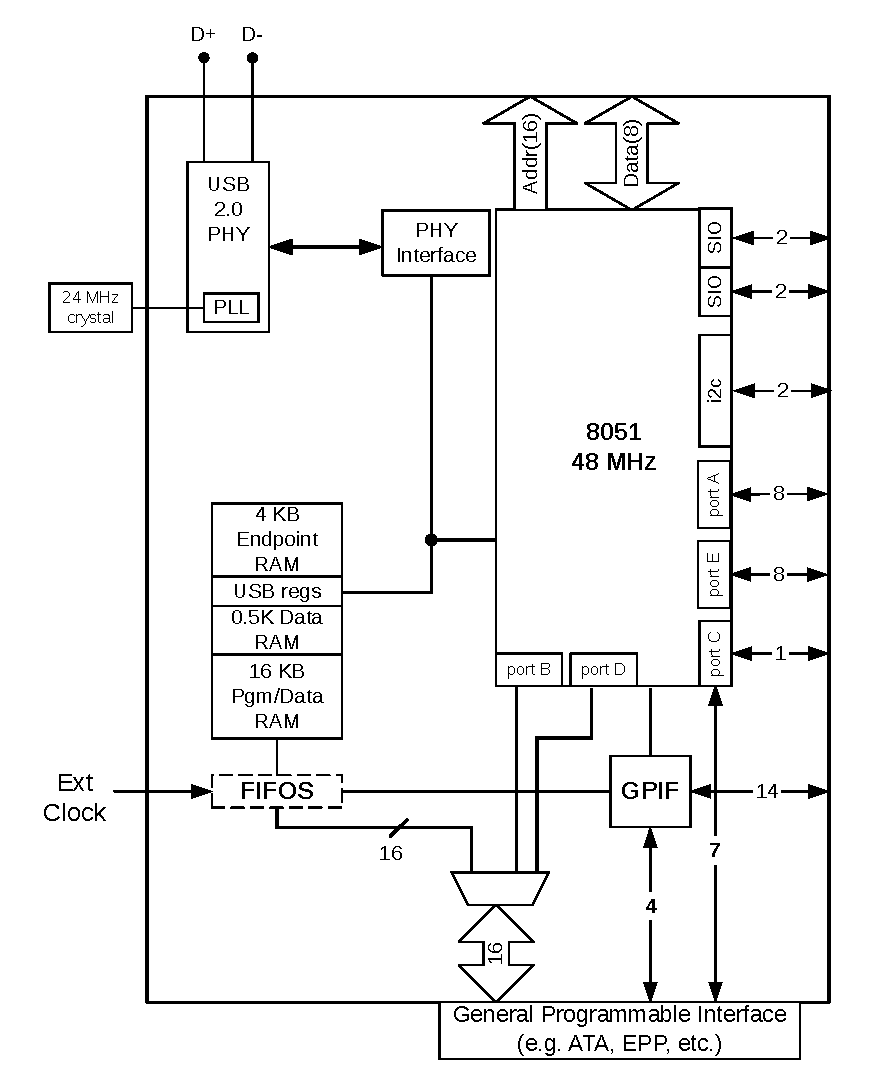
\includegraphics[width=.55\textwidth]{arq.eps}
	\caption{Arquitectura FX2LP~\cite{CypressSemiconductor2014fx2lp}} 
	\label{arqEzUSB}
\end{figure}

La GPIF está pensada principalmente para poder utilizar sistemas que deban ser comandados en forma externa, como por ejemplo un registro de desplazamiento. Por su parte, la memoria FIFO posee \SI{4}{\kilo\byte} de capacidad reservados para almacenar los datos que se intercambian y se destina a aquellos sistemas que pueden proveer las señales de control, aunque también puede ser comandada por el GPIF. Con estas interfaces se posibilita la conexión con casi cualquier dispositivo, ya sea estandarizado (ATA, PCMCIA, EPP, etc) o personalizable (DSP, FPGA, $\mu$C);

%El usuario puede trasmitir datos desde y hacia el Host a través del mismo puerto USB. Sin embargo, también posee dos puertos USART ((acrónimo de Transmisión y Recepción Asíncrona en Serie Universal, en inglés)) que permiten comunicarse con la PC y facilitan en gran medida la tarea de depuración del desarrollo.

%En cuanto a la interfaz con uno o mas periféricos, el controlador posee un puerto $I^2C$, una interfaz de propósito general (GPIF), para sistemas que necesitan ser comandados en forma externa; y una interfaz con memorias FIFO esclavas, a través de las cuales se puede conectar sistemas que cumplen un rol activo en el envío y recepción de información. Estas tres interfaces posibilitan la conexión de dispositivos que poseen tanto puertos estandarizados (ATA, PCMCIA, EPP, etc.), cómo personalizables (DSP, FPGA, microcontroladores, etc).

%Variante 1
 
%El usuario puede trasmitir datos desde y hacia el anfitrión a través del mismo puerto USB, o bien via RS-232. Para comunicarse con sistemas periféricos se puede aprovechar el puerto $I^2C$, la interfaz de propósito general, que actúa como maestro y a la cual se le puede acoplar un periférico esclavo, y/o las memorias FIFO en modo esclavo que puede ser conectada a un sistema maestro. Esto brinda muchas alternativas, desde la conexión a puertos estandar, como ser ATA, PCMCIA, EPP, etc. o también la conexión de dispositivos tales como DSP's y FPGA's.\\
%\textbf{\hl{variante 1}}
%\hl{El usuario puede trasmitir datos desde y hacia el anfitrion a traves del mismo puerto USB, o bien via RS-232. Para comunicarse con sistemas perifericos se puede aprovechar el puerto $I^2C$, la interfaz de proposito general, que actua como maestro y a la cual se le puede acoplar un periferico esclavo, y/o las memorias FIFO en modo esclavo que puede ser conectada a un sistema maestro. Esto brinda muchas alternativas de conexion, desde puertos estandar, como ser ATA, PCMCIA, EPP, etc. hasta dispositivos personalizables como DSP's y FPGA's}.%\\

%variante 2
%El flujo de datos posee dos puntas entre las cuales el controlador hace de nexo. Para ello necesita poder comunicarse tanto con el \host como con los periféricos.\\
%
%El intercambio de información con el \host se lleva a cabo a través del mismo puerto USB, objetivo principal de este trabajo. Sin embargo, también posee dos puertos UART que facilitan en gran medida la tarea de depuración del desarrollo.\\
%
%En cuanto a la interfaz con uno o más periféricos, el controlador posee un puerto $I^2C$, una interfaz de propósito general (GPIF), para sistemas que necesitan ser comandados en forma externa; y una interfaz con memorias FIFO esclavas, a través de las cuales se puede conectar sistemas que cumplen un rol activo en el envío y recepción de información.\\

%\textbf{\hl{variante 2}}
%
%\hl{El flujo de datos posee dos puntas (una PC y un FPGA) entre las cuales el controlador cumple el rol de interfaz. Para ello necesita poder comunicarse tanto con el host como con los perifericos.}%\\
%
%\hl{El intercambio de informacion con el HOST se lleva a cabo a traves del mismo puerto USB, objetivo principal de este trabajo. Sin embargo, tambien posee dos puertos UART que facilitan en gran medida la tarea de depuracion del desarrollo.}%\\
%
%\hl{En cuanto a la interfaz con uno o mas perifericos, el controlador posee un puerto $I^2C$, una interfaz de proposito general (GPIF), para sistemas que necesitan ser comandados en forma externa; y una interfaz con memorias FIFO esclavas, a traves de las cuales se puede conectar sistemas que cumplen un rol activo en el envio y recepcion de informacion.}%\\

Bajo el criterio de este autor, el componente de mayor trascendencia en el funcionamiento del controlador FX2LP es el $\mu$C 8051. Es este componente el encargado de configurar los bloques programables y de inicializar todos los registros que determinan la forma en la que el sistema funciona: la frecuencia de trabajo, la gestión de las memorias y el modo en que fluyen los datos son algunas de las tareas que configura el $\mu$C. El firmware es escrito en lenguaje C para microcontroladores. 

La estructura de la interfaz implementada en este trabajo utiliza la memoria FIFO en modo esclavo, es decir, la memoria responde a señales que proporciona un maestro externo sintetizado en un FPGA. Se escogió la frecuencia de funcionamiento del PLL y se configuraron los extremos que intervienen en la comunicación USB y el modo de funcionamiento, por lo que a continuación se explicitan los detalles referidos a la configuración realizada, con lo que se busca aclarar el funcionamiento y que el lector comprenda los fundamentos de las configuraciones que se plasman en el código del firmware.

\subsection{Microcontrolador Cypress 8051 Mejorado}
	Las tareas que ejecuta el controlador FX2LP son llevadas a cabo por un microcontrolador incorporado al circuito integrado. Dicho $\mu$C es una modificación del 8051 desarrollado por Intel, para que sea más veloz en sus tiempos de ejecución y mejore el desempeño del $\mu$C cómo interfaz, mediante la incorporación de registros especiales adicionales.  De esta forma, la manera a través de la cuál el desarrollador elabora la configuración del controlador, es a través de la programación de este $\mu$C 8051.
	
	Para elaborar el firmware que ejecuta el controlador FX2LP, se desarrolló un programa en C para microcontroladores y se compiló mediante el compilador C51 de Keil, a través del entorno de desarrollo integrado Keil $\mu$Vision. Los archivos resultantes de la configuración realizada se pueden encontrar en el Apéndice~\ref{ap:fx2lp}
	
	Cypress provee, dentro del kit de desarrollo CY3684, un conjunto de archivos que contienen código base sobre el cual el desarrollador implementa la configuración. Este conjunto de archivos es denominado framework, el cual posee, entre otras cosas, encabezados con definiciones de macros, constantes, registros, tipos de datos y declaración de funciones prototipo. También incorpora algunas funciones precompiladas para utilizar los periféricos que contiene la placa de desarrollo.
	
	La Figura \ref{int:fw} muestra un diagrama de flujo del firmware que se desarrolló en el presente trabajo. El mismo fue elaborado utilizando la estructura propuesta por Cypress para el desarrollo de la comunicación que se implementó. Se puede observar que al inicio del programa se inicializan variables de estado que corresponden a una máquina de estados, desarrollada por Cypress, que ejecuta las tareas de la comunicación USB. Luego, se invoca una función llamada \verb|TD_Init()|. Esta es la función a través de la cual se implementa la configuración que se desarrolló en este trabajo. En las secciones siguientes se profundiza cada uno de los bloques que intervienen.
	
	Una vez configurado el funcionamiento del controlador, se habilitan las interrupciones, lo que da lugar a que todos los bloques del circuito integrado puedan funcionar e intercambiar información. Seguidamente, el programa entra en un lazo infinito, donde en primer lugar ejecuta la función \verb|TD_Poll()|, en la cual el desarrollador programa las tareas que ejecuta el controlador durante la rutina de funcionamiento. Como segundo paso, el controlador chequea si arribó desde el Host una transferencia de control cuyo PID indique Setup. En caso afirmativo, ejecuta lo solicitado por el Host. En caso contrario, vuelve a ejecutar la función \verb|TD_Poll()|.
	
	\begin{figure}[h]
	\centering
	\begin{tikzpicture}[scale=.75\textwidth/\paperwidth]
	\begin{scope}[transform shape,node distance=1,>=latex]
	\node[mealy]	(start)	[]	{Iniciar: Reset \\ \verb|main();|};
	\node[moore]	(init)	[below=of start]	{Inicia Variables de Estado}
	edge[<-,thick] (start);
	\node[moore]	(us1)	[below=of init]		{\verb|TD_Init();|}
	edge[<-,thick]	(init);
	\node[moore]	(EI)	[below=of us1]	{Habilita\\Interrupciones}
	edge[<-,thick](us1);
	\node[node distance=0.7]			(aux1)	[below=of EI] 	{};
	\draw[<-,thick](aux1.base) to (EI);
	\node[moore,node distance=.5]	(poll)	[below=of aux1]	{\verb|TD_Poll();|}
	edge[<-,thick](aux1.base);
	\node[ask]		(pr1)	[below=of poll]	{Paquete de Setup}
	edge[<-,thick](poll);
	\node[moore]	(setup)	[right=of pr1]	{\verb|SetupComand();|};
	\draw[->,thick] (setup) |- (aux1.base);
	\node[]			(aux2)	[below=of pr1]	{};
	\draw[->,thick]	(pr1) -- node[above,near start]{Si} (setup);
	\draw[thick]	(pr1) -- node[left,near start]{No}	(aux2.base);
	\node[node distance=2.5](aux3)	[left=of aux2] {};
	\draw[thick]	(aux2.base) -- (aux3.base);
	\draw[->,thick]	(aux3.base)	|-	(aux1.base);
	\end{scope}
	\end{tikzpicture}
	\caption{Diagrama en bloques del firmware que ejecuta el $\mu$C de la interfaz}
	\label{int:fw}
\end{figure}

%	Keil μVision es un entorno de desarrollo integrado (IDE). Se entiende por IDE a un software
%	que integra en un entorno gráfico las herramientas que permiten elaborar un programa que
%	ejecutará un procesador, desde la escritura del algoritmo en uno o más lenguajes, su compilación,
%	las pruebas y el depurado.
%	El programa utilizado posee, entre otras cosas, editor de textos con atajos de teclado,
%	comandos que aceleran la escritura de código y resaltado de palabras claves para diferentes
%	lenguajes de programación, navegador de archivos. También ejecuta, con solo un click, el
%	compilador con la sintaxis correcta, y posee un depurador que, a través de un intérprete, permite
%	ir ejecutando el código lı́nea por lı́nea o en bloques.
%	Para realizar un programa en este entorno, Cypress provee, junto con su framework, un
%	proyecto vacı́o que puede ser copiado y pegado. Sin embargo, se puede realizar la configuración
%	manual. Las instrucciones de este procedimiento se ubican en el Apéndice ??.
%	En cuanto al compilador se refiere, el utilizado es C51. Éste es un programa que otorga
%	un archivo hexadecimal con un código que será ejecutado por microcontroladores que estén
%	implementados con la misma estructura que un Intel 8051, cómo lo es el microcontrolador que
%	posee el FX2LP.
\subsection{Frecuencia de trabajo del sistema}
	La configuración principal del sistema se realiza a través de la función \verb|TD_Init()|. El primer módulo que configura es el PLL ({\it Phase-Locked Loop}). Un PLL es un lazo de servocontrol cuyo parámetro controlado es la fase de una réplica, generada en forma local, de una señal de entrada~\cite{Sklar2001}. En otras palabras, permite obtener dos señales iguales a través de un detector de fase. Si se incorpora un contador entre la señal generada y la entrada del comparador de fase, la señal generada tendrá una frecuencia igual al producto de la entrada por el recorrido del contador. Si, en cambio, se coloca el contador a la salida del PLL, la frecuencia puede ser dividida. Así, es posible obtener señales de frecuencia modificable.

	El PLL incorporado en el controlador permite elevar la frecuencia de un cristal de \SI{24}{\mega\hertz} hasta los \SI{480}{\mega\hertz} que necesita el transceptor USB para el cumplimiento de la norma USB. A su vez, a través de un divisor de frecuencias, permite seleccionar diferentes frecuencias de trabajo del $\mu$C 8051, entre \si{12}, \si{24} o \SI{48}{\mega\hertz}.
	
	A través de los bits especiales CLKSPD[1:0] del registro de Control y Estado de CPU (CPUCS). En la implementación realizada, se seleccionó la frecuencia de trabajo del $\mu$C a \SI{48}{\mega\hertz}.
	
	\begin{lstlisting}[language=C,backgroundcolor=\color{gray!30}]
	//CPUCS - Registro de Control y Estado del CPU
	//	CLKSPD[1:0] -> "00" => 12 MHz
	//				-> "01" => 24 MHz
	//				-> "10" => 48 MHz
	CPUCS = ((CPUCS & ~bmCLKSPD) | bmCLKSPD1); // 48 MHz
	\end{lstlisting}	

\subsection{Memoria FIFO}
	El controlador FX2LP posee una sección especial de memoria destinada al almacenamiento de los datos que fluyen desde cada uno de los extremos de la comunicación. A esta memoria pueden acceder tanto los componentes del propio controlador, como también los periféricos que se comunican a través de él. Desde el punto de vista de la electrónica digital, cada uno de los componentes que acceden a esta memoria pueden tener diferentes fuentes de señal de reloj. Para salvar los inconvenientes que puede acarrear el uso de sistemas con fuentes de reloj independientes, esta porción de memoria reservada es de tipo FIFO. Debido a que se puede acceder a estas memorias FIFO tanto desde el interior de controlador FX2LP, como desde el exterior, deben ser configuradas en ambos sentidos.
	
	La memoria FIFO puede ser programada y configurada de diferentes formas, en función de los requerimientos sistemas periféricos acoplados a ella. Cada uno de los periféricos conectados a la memoria FIFO se denomina extremo o EP\footnote{EP es una abreviación del término inglés {\it endpoint}, que significa ``Extremo''. Esto quiere decir que cada uno de los periféricos conectados a la memoria FIFO es un extremo de la comunicación.}. Las características a configurar son el tamaño (\si{64}, \si{512} o \SI{1024}{\byte}), la cantidad de bloques o partes en que se divide la memoria (puede estar dividida hasta en 4 extremos) y la cantidad de buffers de datos utilizados para almacenar los datos de cada bloque de memoria.
	
	Los buffers son porciones de memoria físicamente separadas pero que, en la operación, el controlador puede intercambiar de forma tal que se acceda a ellos a través de una misma dirección de memoria. El uso de buffers múltiples implica que un EP utiliza más de un buffer. Los buffers múltiples poseen la función de evitar la congestión de datos. Con doble buffer, un periférico coloca o extrae datos del buffer de un EP, mientras el $\mu$C, utiliza otro del mismo EP. La selección del buffer donde cada componente escribe y/o lee los datos lo asigna e intercambia la interfaz en forma automática. Se pueden configurar también un triple o cuádruple buffer, lo que agrega sendas porciones de memoria extra a la reserva. De esta forma, se le otorga al sistema, en forma simultánea, gran capacidad de datos y ancho de banda.
	
	En este desarrollo, se configuró la memoria FIFO con dos EP. El EP2\footnote{EPx será un extremo con dirección x, siendo x un número entero. En este caso, EP con dirección 2.}, es un EP de entrada (envía datos al Host). Requiere una gran cantidad de datos, debido a que será por donde los sensores transmitirán todos los datos que adquieran. Además, es necesario que posea una buena cantidad de almacenamiento de datos y que estos datos sean enviados de la forma más rápida posible. Por tanto, el EP2 se configuró con dos buffers de \SI{1024}{\byte}, para que efectúe transferencias isócronas.
	
	Por su parte, se configura el EP8 como EP de salida (recibe datos desde el Host). Este EP se utiliza para recibir la configuración de los sensores, que se espera que sea de menor cantidad y más distanciada en el tiempo que los datos adquiridos. Se configuró, entonces, con dos buffers de \SI{512}{\byte} para transferencias en masa.
	
	Debido a que la memoria FIFO cumple el rol de interfaz entre los periféricos y el módulo del controlador FX2LP que efectúa las tareas propias de la comunicación USB, la configuración de dicha memoria se efectúa por separado, conteniendo información relevante a cada etapa de la comunicación.
	
\subsubsection{Interfaz hacia los periféricos}
	Cypress provee varias interfaces para comunicar el controlador hacia los periféricos. I$^2$C y UART son dos posibilidades, aunque poseen un ancho de banda muy limitado. La interfaz que opera con mayor ancho de banda es la memoria FIFO. Esta puede ser utilizadas en modo esclavo, es decir, que un sistema externo comande la lectura y la escritura de datos en ellas, o bien, a través de la interfaz GPIO, puede ser comandada por el $\mu$C 8051. La implementación que se realiza en el desarrollo de la comunicación utiliza la memoria FIFO en modo esclavo.
	
	La frecuencia de funcionamiento de estas interfaz es independiente del reloj del sistema. Puede ser configurado para usar una señal de reloj interna de \si{30} o \SI{48}{\mega\hertz}, propia de la interfaz, o bien, ser provista por un sistema externo al controlador. También, es importante indicarle al controlador si la interfaz funcionará en modo asíncrono. Todos estos parámetros son configurados a través del registro Configuración de Interfaz (IFCONFIG).
	
	La configuración que se realizó en esta implementación, utiliza el reloj interno de la interfaz, corriendo a \SI{48}{\mega\hertz}. Además, se indica que las memorias FIFO esclavas son utilizadas en modo asincrónico. Dicha configuración se plasma en las siguientes líneas de código:
	
	\begin{lstlisting}[language=C,backgroundcolor=\color{gray!30}]
	//IFCONFIG - Registro de Configuración de la Interfaz
	//	b7 	   -> fuente de reloj: '1' interna, '0' externa
	//	b6 	   -> frec: '1' 48 Mhz, '0' 30 MHz
	//	b3 	   -> asinc: '1' asíncrono
	//	b[1:0] -> modo de interfaz: "11" FIFO esclava
	IFCONFIG = 0xCB;
	SYNCDELAY;
	\end{lstlisting}

	El controlador FX2LP posee cuatro pines que emiten señales del estado de las memorias FIFO (comunmente conocidas como ''banderas´´ o \textit{flags}). Dichos pines pueden ser programados para que indiquen si una porción particular de memoria se encuentra vacía, llena o si sobrepasa un nivel programable de datos. También pueden ser configurados para que indiquen el estado completo (vacío, lleno y el nivel programable) de la porción de memoria activa. Cada porción de memoria se activa a través de dos puertos de dirección, comandados por un sistema externo al controlador FX2LP.
	
	Para la comunicación desarrollada, solo son importantes las banderas que indican cuando el EP8 está vacío y que el EP2 está lleno. Si bien no son necesarias, por completitud, también se configuraron las señales que indican que el EP2 está vacío y que el EP8 se encuentra lleno. Cada uno de los \textit{flags} se denominan A, B, C y D y se configuran por pares a través de los registros PINFLAGSAB y PINFLAGSCD, de la forma en que se muestra a continuación.
	
	\begin{lstlisting}[language=C,backgroundcolor=\color{gray!30}]
	PINFLAGSAB = 0xBC;	// FLAGA <- EP2 Full Flag
						// FLAGD <- EP2 Empty Flag
	SYNCDELAY;
	PINFLAGSCD = 0x8F;	// FLAGC <- EP8 Full Flag
						// FLAGB <- EP8 Empty Flag
	\end{lstlisting}
	
	
\subsubsection{Interfaz hacia el módulo de comunicación USB}
	Desde el extremo interno del controlador FX2LP, la memoria FIFO se conecta al Motor de Interfaz Serial (MIS). El MIS es un módulo que se encarga de tomar datos en paralelo y convertilos en una secuencia seriada. Para cumplir con la norma USB, el MIS debe ser capaz de empaquetar, enviar, recibir y desempaquetar toda la información, así como leer los Token que emite el Host, calcular y corroborar los códigos cíclicos de detección de errores y todo lo relacionado al protocolo propiamente dicho. Luego, el transceptor USB efectúa las tareas de codificación y decodificación de los mensajes transmitidos a través del bus.
	
	Para la configuración, es necesario indicarle al controlador FX2LP el funcionamiento que tendrá cada uno de los EP. Los parámetros programables son: si está activo o no, el sentido de la comunicación (sea hacia o desde el Host), el tipo de transferencia, el tamaño de la misma y la cantidad de buffers múltiples que se utilizan. En el desarrollo que se presenta se configura el EP2 como entrada de \SI{1024}{\byte} con dos buffers y el EP8 como salida con dos buffers de \SI{512}{\byte}. También se configura el EP1 con un buffer de \SI{64}{\byte} como entrada y otro igual como salida, ya que viene implementado en una memoria separada dentro del circuito integrado FX2LP y no interfiere con el desempeño pretendido en este trabajo. Los otros EP válidos (EP4 y EP6) no se utilizan, con el objetivo de maximizar la memoria disponible para los datos útiles. De esta forma, la configuración se realiza a través de la siguiente línea de código:
	
	\begin{lstlisting}[language=C,backgroundcolor=\color{gray!30}]
	//EPxCFG - Registros de configuración de extremos
	//	b7 	   -> '1' EP activo
	//	b6 	   -> dir: '0' salida, '1' entrada
	//	b[5:4] -> tipo: "01" => isocronico
	//					"10" => masa
	//					"11" => interrupción
	//	b3 	   -> tamaño: '0' 512 bytes, '1' 1024 bytes
	//	b[1:0] -> buffer: 	"00" => x4
	//						"10" => x2
	//						"11" => x3
	EP1OUTCFG = 0xA0;
	SYNCDELAY;
	EP1INCFG = 0xA0;
	SYNCDELAY;
	// dir:entrada, tipo:isoc, tam:1024, x3
	EP2CFG = 0xDB;
	SYNCDELAY;
	EP4CFG = 0x7F; //Inactivo
	SYNCDELAY;
	EP6CFG = 0x7F; //Inactivo
	SYNCDELAY;
	// dir:salida, tipo:masa, tam:512, x2
	EP8CFG = 0xA2; 
	SYNCDELAY;
	\end{lstlisting}
	
%\subsection{Motor de Interfaz Serial}
%	El Motor de Interfaz Serial (MIS) es un módulo incorporado al circuito integrado que se encarga de tomar datos en paralelo y convertilos en una secuencia seriada.

%	\begin{figure}[ht]%TODO hacer con tikz para que quede prolija
%		\centering
%		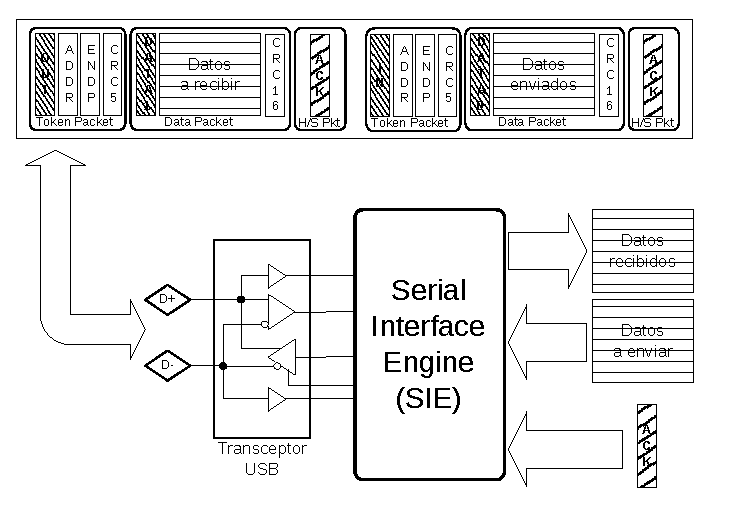
\includegraphics[width=.8\textwidth]{usbxcvr}
%		\caption{Implementación del enlace USB realizado por el EZ-USB~\cite{CypressSemiconductor2014fx2lp}}%TODO(\hl{se copiaria con tikz para mejorar prolijidad})}
%		\label{usbxcvr}
%	\end{figure}
%	
%	La comunicación USB entre el controlador FX2LP y la PC se realiza a través del transceptor, unido al MIS. Para realizar el intercambio de datos, el firmware solo debe colocar o extraer los datos de buffers programables y modificar las banderas de handshaking. En forma automática, el MIS se encargan de empaquetar, enviar, recibir y desempaquetar toda la información, así como leer los tokens que emite el host, calcular y corroborar los códigos cíclicos de detección de errores y todo lo relacionado al protocolo propiamente dicho. El transceptor codifica y decodifica todo a nivel físico.%\\
%	
%	La Figura \ref{usbxcvr} muestra la función del MIS. Toma los datos colocados en los buffers de extremos, agrega la información que corresponde al encabezado y a la cola y, finalmente, coloca el registro de handshaking. Esto último, se observan como ACK (abreviación del ingles {\it acknowledge}, que significa reconocer, aceptar o agradecer) en la Figura \ref{usbxcvr}. En el extremo del controlador, estas banderas se colocan en un registro especial que indica si el sistema está disponible, si los datos fueron colocados o leídos, dependiendo el caso tratado.

%\subsection{Modo}		
%\subsection{Buffers de extremos}
%	El MIS guarda los datos que aún no han sido enviados y/o los que han sido recibidos pero no leídos por ningún periférico en una memoria RAM específica, denominada buffer de extremo.%\\
%	
%	La norma USB define a un dispositivo extremo como una porción exclusiva e identificable de una dispositivo USB que es fuente o un sumidero de información. En otras palabras, USB ve a cada extremo como una memoria FIFO de donde surge o finaliza la información. En ingles, el termino extremo recibe el nombre de {\it endpoint}, por lo que, en adelante, cuando se hable de ellos se abreviara como EP o EPx, siendo la x un número que indica la dirección del extremo.%\\
%	
%	La serie de controladores FX2LP dispone de hasta 7 EP programables, los cuales deben poseer al menos dos buffers. La norma USB indica que cualquier dispositivo USB debe poseer un EP con dirección 0 que se destina para control y configuración, por lo que el controlador está dotado de \SI{64}{\byte} para este fin. Es el único EP que puede ser bidireccional en el sentido del flujo de datos. A través de él, host y dispositivo envían y reciben transferencias de control. Luego, se incorporan dos EP1, que poseen un buffer de \SI{64}{\byte} cada uno. Estos EP se identifican por la dirección de los datos, ya que uno de ellos es de salida y el otro de entrada de datos.%\\
%	
%	\begin{figure}[t]
%		\centering
%		\begin{tikzpicture}[scale=.7*\textwidth/\paperwidth,node distance=2.7]
%			\begin{scope}[transform shape]
%				\begin{scope}[node distance=0.4]
%					\node[buf]	(ep2b1)	[anchor=north]		{\ep{1}{2}{512}};
%					\node[buf]	(ep2b2)	[below=of ep2b1]	{\ep{2}{2}{512}};
%					\node[obuf]	(ep4b1) [below=of ep2b2]	{\ep{1}{4}{512}};
%					\node[buf]	(ep4b2) [below=of ep4b1]	{\ep{2}{4}{512}};
%					\node[obuf]	(ep6b1)	[below=of ep4b2]	{\ep{1}{6}{512}};
%					\node[buf]	(ep6b2)	[below=of ep6b1]	{\ep{2}{6}{512}};
%					\node[obuf]	(ep8b1)	[below=of ep6b2]	{\ep{1}{8}{512}};
%					\node[buf]	(ep8b2)	[below=of ep8b1]	{\ep{2}{8}{512}};
%				\end{scope}
%				
%				\begin{scope}[node distance=0.4, xshift=90]
%					\node[buf]	(ep2b3)	[anchor=north]		{\epg{1}{2}{1024}};
%					\node[obuf] (ep2b4)	[below=of ep2b3]	{\epg{2}{2}{1024}};
%					\node[obuf]	(ep2b5)	[below=of ep2b4]	{\epg{3}{2}{1024}};
%					\node[obuf]	(ep8b3)	[below=of ep2b5]	{\ep{1}{8}{512}};
%					\node[buf]	(ep8b4)	[below=of ep8b3]	{\ep{2}{8}{512}};
%				\end{scope}
%			\end{scope}
%		
%			\begin{scope}[on background layer]
%				rounded corners,]
%				\node[env, fit=(ep2b1)(ep2b2)]			(ep21)	{};
%				\node[env, fit=(ep4b1)(ep4b2)]			(ep41)	{};
%				\node[env, fit=(ep6b1)(ep6b2)]			(ep61)	{};
%				\node[env, fit=(ep8b1)(ep8b2)]			(ep81)	{};
%				\node[env, fit=(ep2b3)(ep2b4)(ep2b5)]	(ep22)	{};
%				\node[env, fit=(ep8b3)(ep8b4)]			(ep82)	{};
%				\node[draw=black,fit=(ep21)(ep82)](marco){};
%			\end{scope}
%		
%			\begin{scope}[transform shape]
%				\draw (marco.north) to (marco.south);
%				\node[left=of ep2b1.north east,anchor=north east](add1)	{0xF000};
%				\node[left=of ep2b1.south east,anchor=south east](add2)	{0xF1FF};
%				\node[left=of ep2b2.north east,anchor=north east](add3)	{0xF200};
%				\node[left=of ep4b1.north east,anchor=north east](add4)	{0xF400};
%				\node[left=of ep6b1.north east,anchor=north east](add5)	{0xF800};
%				\node[left=of ep8b1.north east,anchor=north east](add6)	{0xFC00};
%				\node[left=of ep8b2.south east,anchor=south east](add7)	{0xFFFF};
%				\draw[dashed] (add1.north west) to (add1.north west -| marco.east);
%				\draw[dashed] (add3.north west) to (add3.north west -| ep21.east);
%				\draw[dashed] (add4.north west) to (add4.north west -| marco.east);
%				\draw[dashed] (add5.north west) to (add5.north west -| marco.east);
%				\draw[dashed] (add6.north west) to (add6.north west -| marco.east);
%				\draw[dashed] (add7.south west) to (add7.south west -| marco.east);
%			\end{scope}
%	\end{tikzpicture}
%	\caption{Buffers de extremos con sus direcciones de memoria. El cuadro de la izquierda muestra la configuración por defecto. El derecho, la implementada en este trabajo.}
%	\label{epbuf}
%	\end{figure}
%	
%	Finalmente, se incorpora una memoria de \SI{4}{\kibi\byte} que debe ser configurada para los EP2, EP4, EP6 y EP8. La configuración de los EP la realiza el microcontrolador una vez que su programa se encuentra en ejecución. Las variables, conforme a los requerimientos de ancho de banda y acceso al bus son:
%	
%	\begin{itemize}
%		\item Tamaño: Dependiendo del extremo a configurar puede ser de 512 o 1024 bytes.
%		\item Tipo de acceso al bus: Definido según la norma USB, este tipo puede ser por bultos, isócrono o de interrupción. No se admiten en estos EP paquetes de control.
%		\item Cantidad de buffers: Dependiendo del extremo, puede ser dos, tres o cuatro buffers por extremo.
%		\item Habilitación: Se debe indicar al sistema si los extremos se usan o no. El EP no valido, no responderá a un pedido de entrada o salida.
%	\end{itemize}
%	
%	La Figura \ref{epbuf} muestra solo dos de las posibles configuraciones de los EP. A la izquierda se observa la configuración por defecto del controlador FX2LP. Esto es, los cuatro EP habilitados, con 512 bytes cada uno, buffers dobles y comunicación por bultos. A la derecha se muestra la configuración elegida para este trabajo, es decir, solo son EP válidos el EP2 y EP8. EP2 posee tres buffers de 1024 bytes y el EP8 dos buffers con 512 bytes de capacidad cada uno. Siempre se debe considerar que se dispone hasta \SI{4}{\kibi\byte} de memoria.%\\
%	
%	La característica de los buffers múltiples evita la congestión de datos. Con doble buffer, un periférico (o el microcontrolador) coloca o extrae datos de un buffer, mientras otro, del mismo EP, se encuentra enviando o recibiendo datos mediante el MIS. Cuando se configura un triple o cuádruple buffer, se agrega una o dos porciones mas de memoria a la reserva, respectivamente. De esta forma, se le otorga al sistema una gran capacidad de datos y ancho de banda.%\\
%	
%	Un detalle importante de los buffers múltiples es que, a la vista del controlador y/o de un periférico, el buffer posee una sola y única dirección y, es la propia interfaz FX2LP quien se encarga de seleccionar el buffer que corresponde en cada caso. Esto quiere decir que, por ejemplo, teniendo 4 buffers de \SI{512}{\byte} cada uno, el 8051 verá solo uno de \SI{512}{\byte}, sin necesidad de identificar a traves de su firmware con cuál de los cuatro está trabajando.
%	
%\subsection{Memorias FIFO esclavas}
%	\label{cy:fifo}
%	Desde el punto de vista de la electrónica digital, el MIS es un dispositivo que recibe y envía datos desde y hacia el puerto USB utilizando una señal de reloj de \SI{24}{\mega\hertz}. Esta señal, es provista por un cristal de cuarzo incorporado en el circuito impreso del Kit de Desarrollo CY3684 EZ-USB FX2LP. Por su parte, un sistema externo puede o no proveer una señal de reloj y manejo de datos propio cuy a fuente de reloj es a priori desconocida por quien configura el circuito integrado. El controlador USB incorpora memorias FIFO que se encargan de proveer una interfaz entre el MIS y un dispositivo externo, salvando el problema de poseer dos relojes diferentes e independientes.%\\
%	
%	Estas memorias funcionan en modo esclavo, es decir, se debe conectar un dispositivo capaz de proveer una lógica maestra externa que comande la entrada y salida de datos desde una memoria FIFO hacia o desde el exterior. Para los fines del presente trabajo, este modo de funcionamiento es óptimo ya que, dotando al FPGA de una máquina de estados, se logra la transferencia de datos en los tiempos requeridos.%\\
%	
%	El sistema de bus permite conectar a estas memorias hasta cuatro dispositivos diferentes. Por esto, existe un registro que permite seleccionar una porción de memoria FIFO para cada uno de los EP programables en el buffer de extremos.%\\
%	
%	\begin{figure}[ht]
%		\centering
%		\begin{tikzpicture}[scale=1*\textwidth/\paperwidth]
%			\begin{scope}[transform shape,node distance=4,>=latex]
%				\node[simple]	(fifo)		[]	 			{FIFO's Esclavas};
%				\node[simple]	(master)	[right=of fifo]	{Maestro Externo};
%				\draw[<->,thick]	([yshift=5*110/6]fifo.east) --node [above]{IFCLK} ([yshift=5*110/6]master.west);
%				\draw[<->,thick]	([yshift=4*110/6]fifo.east) --node [above]{FD[15:0]} ([yshift=4*110/6]master.west);
%				\draw[<-,thick]	([yshift=3*110/6]fifo.east) --node [above]{FIFOADR[1:0]} ([yshift=3*110/6]master.west);
%				\draw[->,thick]	([yshift=2*110/6]fifo.east) --node [above]{FLAGA} ([yshift=2*110/6]master.west);
%				\draw[->,thick]	([yshift=1*110/6]fifo.east) --node [above]{FLAGB} ([yshift=1*110/6]master.west);
%				\draw[->,thick]	([yshift=0*110/6]fifo.east) --node [above]{FLAGC} ([yshift=0*110/6]master.west);
%				\draw[->,thick]	([yshift=-1*110/6]fifo.east) --node [above]{FLAGD} ([yshift=-1*110/6]master.west);
%				\draw[<-,thick]	([yshift=-2*110/6]fifo.east) --node [above]{SLOE} ([yshift=-2*110/6]master.west);
%				\draw[<-,thick]	([yshift=-3*110/6]fifo.east) --node [above]{SLWR} ([yshift=-3*110/6]master.west);
%				\draw[<-,thick]	([yshift=-4*110/6]fifo.east) --node [above]{SLRD} ([yshift=-4*110/6]master.west);
%				\draw[<-,thick]	([yshift=-5*110/6]fifo.east) --node [above]{PKTEND} ([yshift=-5*110/6]master.west);
%			\end{scope}				
%		\end{tikzpicture}
%		\caption{Puertos de interfaz entre las FIFO's y un maestro externo}
%		\label{interfazfifo}
%	\end{figure}
%
%	La Figura \ref{interfazfifo} muestra las señales de la interfaz entre las memorias FIFO's y un maestro esclavo. Estas son:
%	
%	\begin{itemize}
%		\item IFCLK: señal de reloj. No es necesario en caso de conectar la interfaz en modo asincrónico. La señal de reloj puede ser provista por el controlador o por el dispositivo de control en forma programable.
%		\item FD[15:0]: constituye el bus de datos. Según se programe, este puede ser de 8 o 16 bits, en forma independiente para cada EP.
%		\item FIFOADDR[1:0]: puerto de direcciones. A través de él se selecciona la memoria activa en el bus.
%		\item FLAGx: Los cuatro puertos de flag son configurables e indican memoria llena, vacía o un nivel programable. También pueden indicar el estado de una memoria específica o de la que se encuentra activa a través de FIFOADDR.
%		\item SLOE, SLWR, SLRD: son las señales de control. A través de ellas el maestro entrega las ordenes de lectura y escritura.
%		\item PKTEND: a través de este puerto el maestro indica que terminó una transferencia de datos.
%	\end{itemize}

\subsection{Modos de entrada y salida automáticos}
	
	Los datos se reciben o envían a través del MIS. Dichos datos, pueden ser enviados en forma automática desde y hacia las memorias FIFO, o bien, pueden ser dirigidos hacia el $\mu$C, el cual debe dirigir los datos desde y hacia su destino (el MIS o las memorias). Esto último permite leer, modificar, suprimir, agregar y/o generar nuevos datos antes de ser remitidos a su destinatario. Estos caminos se pueden ver en la Figura \ref{modesfifo}.%\\
	
	Aunque el envío de datos se hace siempre de forma automática, el fabricante llama a estos caminos "MODO MANUAL", en caso de enviar los datos a través del $\mu$C 8051, y "MODO AUTOMÁTICO", cuando la comunicación es directa entre el MIS y las FIFO. Además, se programan en forma independiente para cada extremo, sea este de salida o entrada. Es decir, la entrada de un EP puede ser manual y la entrada de otro puede ser automática.%\\
	
	Se debe notar en la Figura \ref{modesfifo} que se refiere a paquetes de entrada cuando estos poseen una dirección que se inicia en un periférico y termina en el host y de salida cuando llevan el sentido contrario. Esto se debe al rol central que ejerce el host en la comunicación USB.
	
	\begin{figure}[b]
		\centering
		\begin{tikzpicture}[scale=0.8\textwidth/\paperwidth,text width=5em,align=center,>=latex,node distance=38mm]		
			\begin{scope}[transform shape]
				\node[interior]	(mis)									{MIS};
				\node			(im)	[right=of mis]					{};
				\node[interior]	(uc)	[above=of im]					{$\mu$C};
				\node[interior] (fifo)	[right=of im,text width=4em]	{FIFOs Esclavas};
				\node			(et)	[left=of uc]					{FX2LP};
				
				\draw[->]([xshift=1.5mm]fifo.north)to node[above,mode text]{MODO ENTRADA MANUAL} ([yshift=1mm]uc.east);
				\draw[->]([yshift=1mm]uc.west)to node[above,mode text]{MODO ENTRADA MANUAL}([xshift=-1.5mm]mis.north);
				\draw[->] ([yshift=-1mm]uc.east)to node[below,mode text]{MODO SALIDA MANUAL}([xshift=-1.5mm]fifo.north);
				\draw[->]([xshift=1.5mm]mis.north)to node[below,mode text]{MODO SALIDA MANUAL}([yshift=-1mm]uc.west);
				
				\draw[->]([yshift=1mm]fifo.west)to node[above,mode text]{MODO AUTO ENTRADA}([yshift=1mm]mis.east);
				\draw[->]([yshift=-1mm]mis.east)to node[below,mode text]{MODO AUTO SALIDA}([yshift=-1mm]fifo.west);
				
				\node[exterior]	(pc)	[left=of mis]	{Host};
				\draw[->]([yshift=1mm]mis.west)to([yshift=1mm]pc.east);
				\draw[->]([yshift=-1mm]pc.east)to([yshift=-1mm]mis.west);
				
				\node[exterior]	(fpga)	[right=of fifo]	{Maestro Externo};
				\draw[->]([yshift=1mm]fifo.east)to node[above]{Banderas}([yshift=1mm]fpga.west);
				\draw[<-]([yshift=-1mm]fifo.east)to node[below]{Control}([yshift=-1mm]fpga.west);
				\end{scope}	
				
				\begin{scope}[on background layer]
				\node(fx)[rounded corners,fill=black!10,fit=(mis)(uc)(fifo)(et)]{};
			\end{scope}
		\end{tikzpicture}
		\caption{Modos de conexión de la memoria FIFO, el microntrolador y el MIS}
		\label{modesfifo}
	\end{figure}

	Para efectuar la configuración del modo de funcionamiento de cada EP, se recurre a los Registros de Configuración Extremo-FIFO esclava (EPxFIFOCFG). A continuación se muestra la programación efectuada en este trabajo, en donde se envían los datos en forma automática, tanto de entrada como de salida. Se debe notar que la activación del modo automático se produce por el flanco ascendente de la variable de configuración, por lo que primero se coloca el registro en cero y luego se establece el valor de la configuración. También se indica en este registro que los datos tendrán un ancho de 16 bits.
	
	\begin{lstlisting}[language=C,backgroundcolor=\color{gray!30}]
	//EPxFIFOCFG - Registro de configuracion extremo/FIFO
	//	b6	->	'1' Indica lleno un byte antes
	//	b5	->	'1' Indica vacío un byte antes
	//	b4	->	'1' Modo Auto Salida
	//	b3	->	'1' Modo Auto Entrada
	//	b2	->	'1' Permite paquetes de entrada con largo 0
	//	b0	->	'1' bus de 16 bits, '0' bus de 8 bits
	EP8FIFOCFG = 0x00;
	SYNCDELAY;
	EP2FIFOCFG = 0x00;
	SYNCDELAY;
	
	//establecer modo auto. se necesita flanco ascendente
	EP8FIFOCFG = 0x11;
	SYNCDELAY;
	EP2FIFOCFG = 0x0D;
	SYNCDELAY;
	\end{lstlisting}
	
	Una vez configuradas las interfaces, se deben restablecer las memorias FIFO, a fin de asegurarse que se encuentran vacías para iniciar la comunicación, a través del registro FIFORESET. El bit 7 de este registro le indica al MIS que la memoria FIFO no se encuentra disponible, y el MIS, a su vez, lo indica al Host si es necesario. Luego, a través de los cuatro bits menores se indica la dirección del EP a restablecer. Finalmente, libera la memoria y se le indica la situación al MIS.
	
	\begin{lstlisting}[language=C,backgroundcolor=\color{gray!30}]
	//FIFORESET - Registro de restablecimiento FIFO
	//	b8		->	'1' Desabilitado
	//	b[3:0]	->	'1' Direccfión de EP
	FIFORESET = 0x80;
	SYNCDELAY;
	FIFORESET = 0x82;
	SYNCDELAY;
	FIFORESET = 0x84;
	SYNCDELAY;
	FIFORESET = 0x86;
	SYNCDELAY;
	FIFORESET = 0x88;
	SYNCDELAY;
	FIFORESET = 0x00;
	SYNCDELAY;
	//establecer modo auto. se necesita flanco ascendente
	EP8FIFOCFG = 0x11;
	SYNCDELAY;
	EP2FIFOCFG = 0x0D;
	SYNCDELAY;
	\end{lstlisting}
	

	En las líneas de código mostradas hasta acá se utiliza el macro {\it SYNCDELAY}. Dicho macro es una secuencia de espera requerida por Cypress para cumplir con los tiempos de mantenimiento asociados a la escritura y lectura de determinados registros~\cite{CypressSemiconductor2014fx2lp}.%, los cuales se explicitan en el Anexo \ref{an:syncdelay}.

		\subsection{Selección de los componentes del sistema}
			\begin{frame}{Selección de la Interfaz USB}
	\alert<2>{Cypress FX2LP}
	\begin{columns}
		\begin{column}{.4\textwidth}
			\includegraphics[width=\textwidth]{fx2lp}
		\end{column}
		\begin{column}{.6\textwidth}
			\begin{itemize}
				\item Pros
				\begin{itemize}
					\item Comunicación paralela de 16 bits
					\item Microcontrolador 8051
				\end{itemize}
				\item Contras
				\begin{itemize}
					\item Requiere esfuerzo en la configuración y software dedicado
				\end{itemize}
			\end{itemize}
		\end{column}
	\end{columns}
		
	FTDI FT4222H
	\begin{columns}
		\begin{column}{.4\textwidth}
			\includegraphics[width=\textwidth]{ft4222h}
		\end{column}
		\begin{column}{.6\textwidth}
			\begin{itemize}
				\item Pros
				\begin{itemize}
					\item No requiere programación
					\item Económico
				\end{itemize}
				\item Contras
				\begin{itemize}
					\item Solo permite Transferencias en Masa
					\item Comunicación SPI cuádruple
				\end{itemize}
			\end{itemize}
		\end{column}
	\end{columns}
\end{frame}

\begin{frame}{Selección del FPGA}
	\centering
	\begin{tikzpicture}[scale=1,>=latex]
		\begin{scope}[transform shape,node distance=2]
			\node[bloque]	(cy)				{Interfaz\\\alert{Cypress\\FX2LP}};
			\node[bloque]	(fpga)	[right=of cy]{FPGA};
			\node[bloque]	(pc) 	[left=of cy]	{PC};
			\draw[->,thick] (pc.15) -- node (usbd+) [above]	{D+} (pc.15 -| cy.west);
			\draw[->,thick] (cy.195) -- node (usbd-) [below]	{D-} (cy.195 -| pc.east);
			\draw[<->,thick] (cy.15) -- node (data) [above] {Datos} (cy.15 -| fpga.west);
			\draw[->,thick]  (fpga.195) -- node (ctrl) [below] {Control} (fpga.195 -| cy.east);
			\node[node distance=.4,text=blue] (usb text) [above=of usbd+] {USB};
		\end{scope}
		\begin{scope}
			\node[rectangle,rounded corners,draw=blue,dashed,fit=(usb text)(usbd+)(usbd-)(cy.south west)(pc.east)](usb){};
		\end{scope}
		\begin{scope}
			\node[draw=blue,ultra thick, ellipse,fit=(fpga)]{};
		\end{scope}
	\end{tikzpicture}
\end{frame}

\begin{frame}{Selección del FPGA}
	\begin{columns}
		\begin{column}{.28\textwidth}
			\centering
			\includegraphics[width=\textwidth]{s3eboard}\\
			\centering
			Spartan-3E Starter\\
			\begin{itemize}
				\item FPGA Spartan 3E de Xilinx
				\item Gran cantidad de periféricos
			\end{itemize}
		\end{column}
		\begin{column}{.28\textwidth}
			\centering
			\includegraphics[width=\textwidth]{nexys3}\\
			\centering
			Nexys 3\\
			\begin{itemize}
				\item FPGA Spartan 6 de Xilinx
				\item Gran cantidad de periféricos
			\end{itemize}
		\end{column}
		\begin{column}{.28\textwidth}
			\centering
			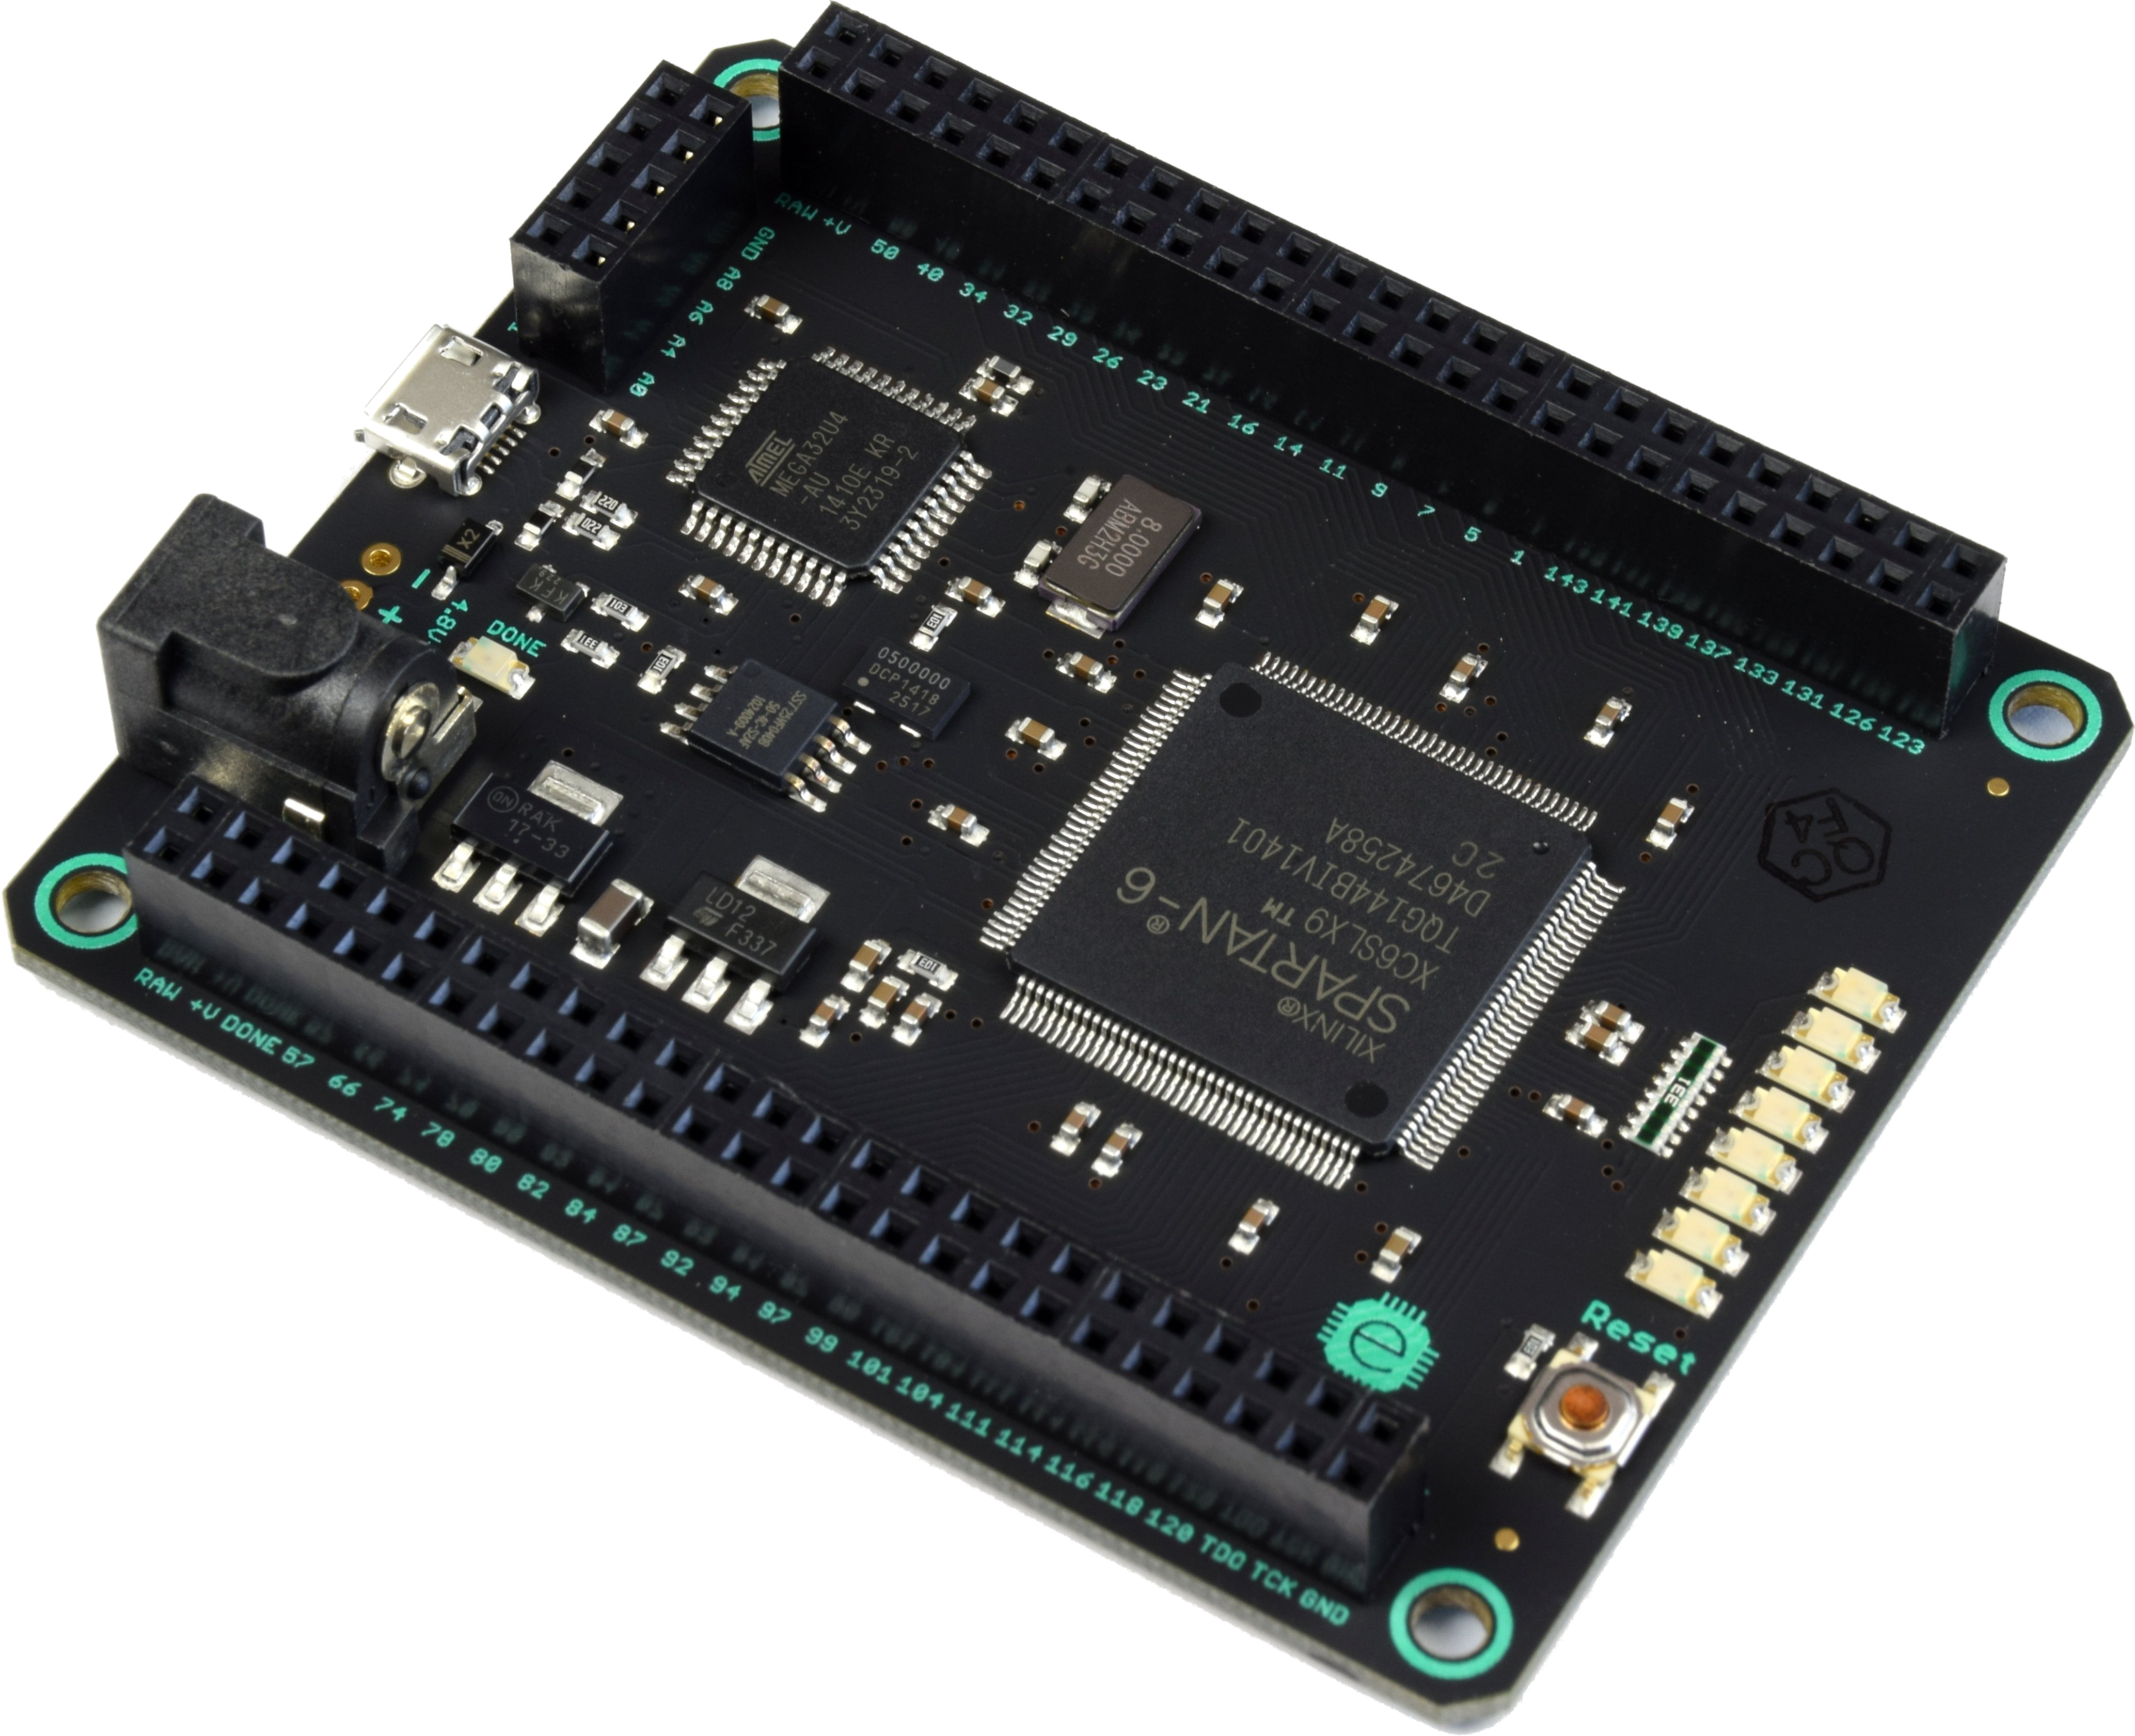
\includegraphics[width=\textwidth]{MojoIso}\\
			\centering
			\alert<2>{Mojo v3\\}
			\begin{itemize}
				\item FPGA Spartan 6 de Xilinx
				\item Muy económica
			\end{itemize}
		\end{column}
	\end{columns}
\end{frame}

\begin{frame}{La placa de desarrollo MOJO v3}
	\begin{columns}
		\begin{column}{.43\textwidth}
			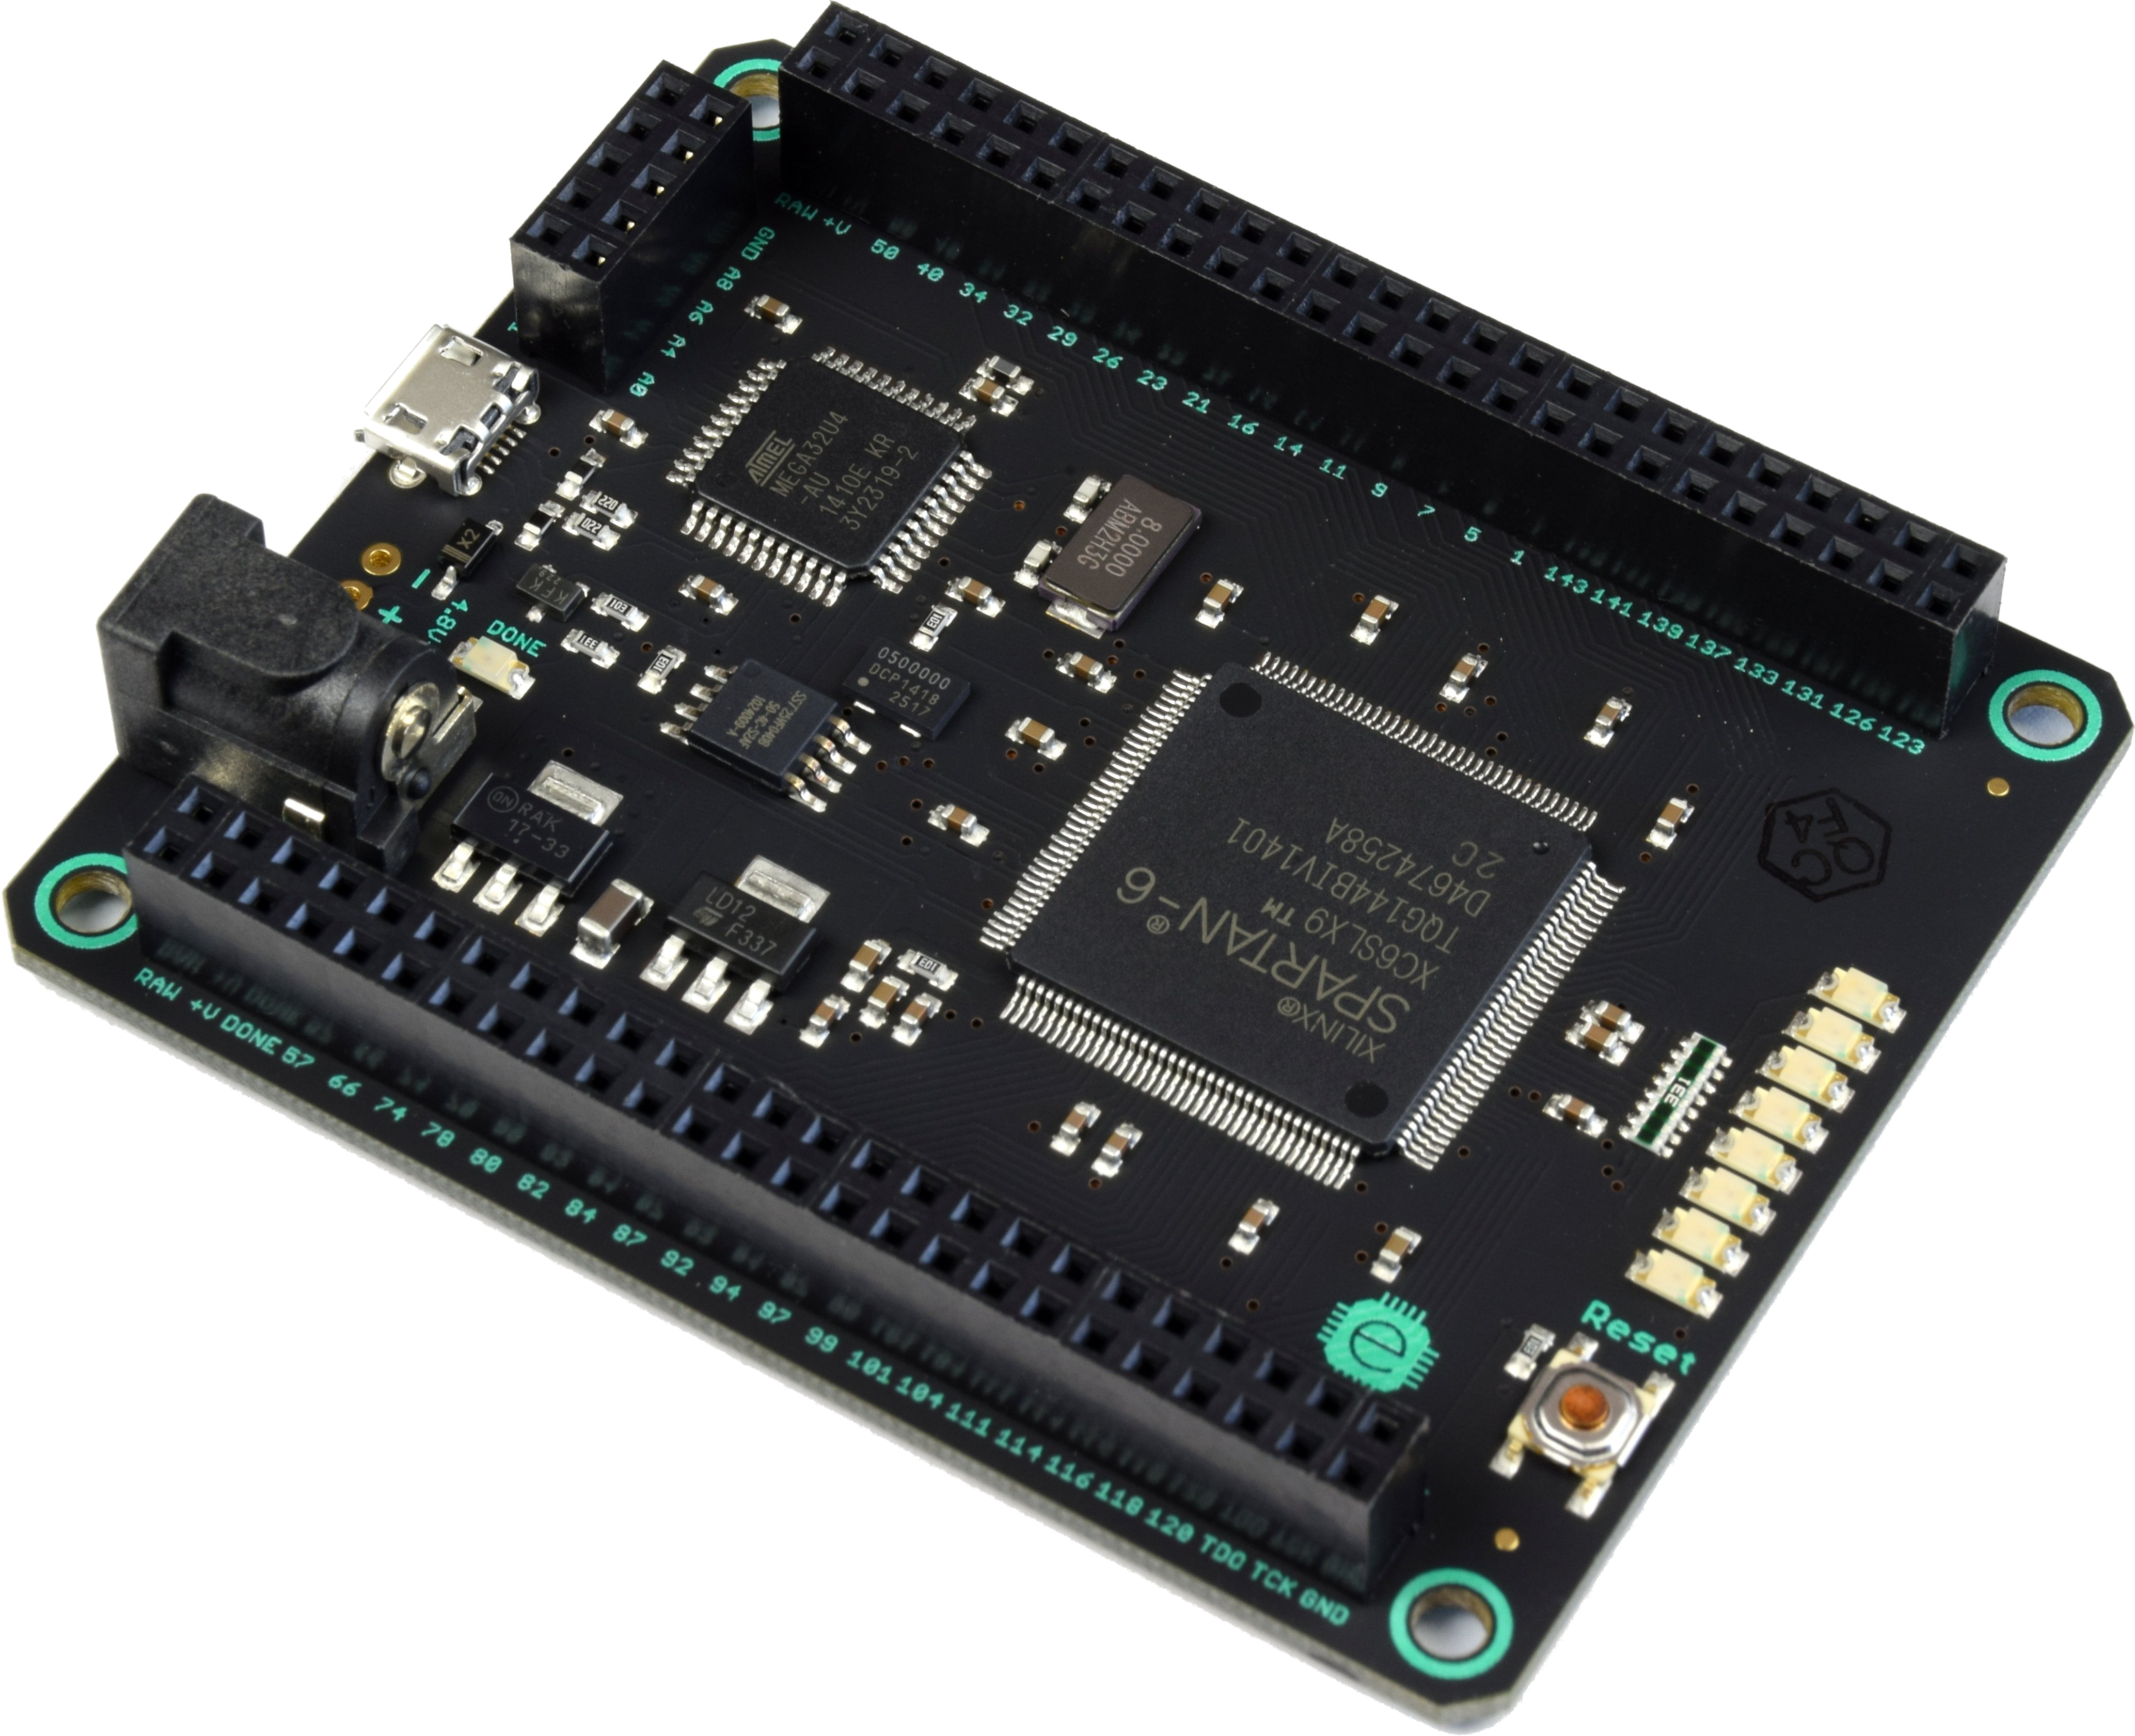
\includegraphics[width=\textwidth]{MojoIso.png}
		\end{column}
		\begin{column}{.55\textwidth}
			\begin{itemize}
				\only<1>{
					\item FPGA Spartan 6 XC6SLX9 de Xilinx
					\item 84 pines IO digitales
					\item 8 entradas analógicas
					\item 8 LEDs de propósito general
					\item 1 pulsador de propósito general
					\item ATmega32U4 para configurar la FPGA y leer los pines analógicos.
					\item Memoria flash para almacenar la configuración de la FPGA.}
				\item USB para programación y comunicación.
				\only<2>{
					\begin{itemize}
						\item USB 2.0 Full-Speed de 12 Mbps
						\item Implementado a través de controlador ATmega32U4
						\item Interfaz FPGA-ATmega32U4 via SPI de 8 Mbps.
					\end{itemize}
				}
			\end{itemize}
		\end{column}
	\end{columns}
\end{frame}

\begin{frame}{Circuito de interconexión}
	\begin{tikzpicture}[scale=1,>=latex]
		\begin{scope}[transform shape,node distance=2]
			\node[bloque]	(cy)				{Interfaz\\\alert{Cypress FX2LP}};
			\node[bloque]	(fpga)	[right=of cy]{FPGA\\\alert{Xilinx Spartan VI}};
			\node[bloque]	(pc) 	[left=of cy]	{PC};
			\draw[->,thick] (pc.15) -- node (usbd+) [above]	{D+} (pc.15 -| cy.west);
			\draw[->,thick] (cy.195) -- node (usbd-) [below]	{D-} (cy.195 -| pc.east);
			\draw[<->,thick] (cy.15) -- node (data) [above] {Datos} (cy.15 -| fpga.west);
			\draw[->,thick]  (fpga.195) -- node (ctrl) [below] {Control} (fpga.195 -| cy.east);
			\node[node distance=.4,text=blue] (usb text) [above=of usbd+] {USB};
			\node[node distance=.5,text width=60,align=center,text=blue] (pcb text)[above=of data]{Placa de\\Interconexión};
		\end{scope}
		\begin{scope}
			\node[rectangle,rounded corners,draw=blue,dashed,fit=(usb text)(usbd+)(usbd-)(cy.south west)(pc.east)](usb){};
			\node[rectangle,rounded corners,draw=blue,ultra thick,fit=(cy.south east)(fpga.north west)(pcb text)](pcb){};
		\end{scope}
	\end{tikzpicture}
\end{frame}

\begin{frame}{Circuito de interconexión}
	\only<1>{
		\begin{itemize}
			\item Versión 1:
		\end{itemize}
		\centering
		\includegraphics[width=.45\textwidth]{63v2anverso}
		\includegraphics[width=.45\textwidth]{64v2reverso}
	}
	\only<2>{
		\begin{itemize}
			\item Versión 2:\\
		\end{itemize}
		\centering
		\includegraphics[width=.45\textwidth]{65v3anverso}
		\includegraphics[width=.45\textwidth]{66v3reverso}
	}
\end{frame}

\begin{frame}{Componentes conectados}
	\centering
	\includegraphics[width=.6\textwidth]{fisico}
\end{frame}

\begin{frame}{Acceso al dispositivo desde la PC}
	\begin{tikzpicture}[scale=1,>=latex]
		\begin{scope}[transform shape,node distance=2]
			\node[bloque]	(cy)				{Interfaz\\\alert{Cypress FX2LP}};
			\node[bloque]	(fpga)	[right=of cy]{FPGA\\\alert{Xilinx Spartan VI}};
			\node[bloque]	(pc) 	[left=of cy]	{PC};
			\draw[->,thick] (pc.15) -- node (usbd+) [above]	{D+} (pc.15 -| cy.west);
			\draw[->,thick] (cy.195) -- node (usbd-) [below]	{D-} (cy.195 -| pc.east);
			\draw[<->,thick] (cy.15) -- node (data) [above] {Datos} (cy.15 -| fpga.west);
			\draw[->,thick]  (fpga.195) -- node (ctrl) [below] {Control} (fpga.195 -| cy.east);
			\node[node distance=.4,text=blue] (usb text) [above=of usbd+] {USB};
			\node[node distance=.5,text width=60,align=center,text=blue] (pcb text)[above=of data]{Placa de\\Interconexión};
		\end{scope}
		\begin{scope}
			\node[rectangle,rounded corners,draw=blue,dashed,fit=(usb text)(usbd+)(usbd-)(cy.south west)(pc.east)](usb){};
			\node[rectangle,rounded corners,draw=blue,dashed,fit=(cy.south east)(fpga.north west)(pcb text)](pcb){};
			\node[ellipse,draw=blue,ultra thick, fit=(pc)]{};
		\end{scope}
	\end{tikzpicture}
\end{frame}

\begin{frame}{Acceso al dispositivo desde la PC}
	Para acceder al puerto USB desde la PC se utilizó la biblioteca libusb-1.0:
	\begin{itemize}
		\item Software libre: Puede ser utilizado sin necesidad de comprar una licencia.
		\item API portable: Permite escribir código que puede ser compilado en múltiples Sistemas Operativos.
		\item Abundante documentación: Se encuentran en Internet manuales y tutoriales muy completos sobre su funcionamiento.
	\end{itemize}
\end{frame}

\begin{frame}{Componentes del sistema}
	\begin{tikzpicture}[scale=1,>=latex]
	\begin{scope}
	\begin{scope}[transform shape,node distance=2]
	\node[bloque]	(cy)				{Interfaz\\\alert{Cypress FX2LP}};
	\node[bloque]	(fpga)	[right=of cy]{FPGA\\\alert{Xilinx Spartan VI}};
	\node[bloque]	(pc) 	[left=of cy]	{PC\\\alert{libusb}};
	\draw[->,thick] (pc.15) -- node (usbd+) [above]	{D+} (pc.15 -| cy.west);
	\draw[->,thick] (cy.195) -- node (usbd-) [below]	{D-} (cy.195 -| pc.east);
	\draw[<->,thick] (cy.15) -- node (data) [above] {Datos} (cy.15 -| fpga.west);
	\draw[->,thick]  (fpga.195) -- node (ctrl) [below] {Control} (fpga.195 -| cy.east);
	\node[node distance=.4,text=blue] (usb text) [above=of usbd+] {USB};
	\node[node distance=.5,text width=60,align=center,text=blue] (pcb text)[above=of data]{Placa de\\Interconexión};
	\end{scope}
	\begin{scope}
	\node[rectangle,rounded corners,draw=blue,dashed,fit=(usb text)(usbd+)(usbd-)(cy.south west)(pc.east)](usb){};
	\node[rectangle,rounded corners,draw=blue,dashed,fit=(cy.south east)(fpga.north west)(pcb text)](pcb){};
	\end{scope}
	\end{scope}
	\end{tikzpicture}
\end{frame}



		\subsection{Configuración de la Interfaz USB}
			\begin{frame}{Placa de desarrollo utilizada para la interfaz}
	\centering
	\includegraphics[height=0.8\textheight]{cy3684}
\end{frame}
\begin{frame}{El circuito integrado FX2LP}
	\centering
	\begin{tikzpicture}[scale=.58,>=latex]
		\begin{scope}[align=center,transform shape]
			\node	(aux1) {};
			\node[core,minimum height=95] (mis)	[left=of aux1,anchor=north east] {MIS};
			\node[core]	(ram) [right=of aux1,anchor=north west,text width=30] {16 kB RAM};
			\node[perif,text width=60] (xcvr) [left=of mis]	{Transceptor USB};
			\node[core,minimum size=60,text width=50] (uc) [above=of aux1] {8051 Mejorado};			
			\node[perif,node distance=2.9] (pll) [left=of uc] {PLL};
			\node	(aux2)	[right=of ram.south]{};				
			\node[core]	(bus)	[right=of aux2,rotate=90,anchor=north west]	{Bus de datos y direcciones};
			\node[perif]	(i2c)	[right=of bus.south east,anchor=north west]	{I2C};
			\node[perif]	(gpif)	[right=of bus.south west,anchor=south west] {GPIF};
			\node[perif,text width=40] (fifo) [below=of gpif] {4 kB FIFO};
			\node 			(aux3)	[right=of fifo]	{};
			\node 			(aux5) 	[left=of ram] {};
			\draw[<->]	(mis) -- (xcvr);
			\draw[<->]	(ram) -- (ram -| mis.east);
			\draw[<->]	(fifo) -- (fifo -| mis.east);
			\draw[<->]	(ram) to (ram -| bus.north);
			\draw[<->]	(uc) to (uc -| bus.north);
			\draw[<-]	(xcvr) to (xcvr |- pll.south);
			\draw[->]	(pll) to (uc);
			\draw[<->]	(i2c) to (i2c -| bus.south);
			\draw[<->]	(gpif) to (gpif -| bus.south);
			\draw[]		(fifo) -| (aux5.center);
		\end{scope}
		\begin{scope}[on background layer]
			\node[contenedor] (fx2) [fit=(pll)(xcvr)(uc)(bus)(mis)(ram)(fifo)(gpif)(i2c)(aux3)]{};
		\end{scope}
		\begin{scope}[transform shape]
			\node[text width=40,align=center]	(xtal)	[left=of pll]{Xtal \SI{24}{\mega\hertz}};
			\node	(host)	[left=3of xcvr]	{PC};
			\draw[<->,ultra thick] (host) -- node [above,text width=70,midway,align=center]{Comunicación USB} (xcvr);
			\draw[->] (xtal) to (pll);
			\draw[<->,ultra thick] (bus.240) -- node [above,align=center,text width=80] {Datos, direcciones y entradas adicionales}(bus.240 -| fx2.east);
			\draw[<->,thick] (gpif) to (gpif -| fx2.east);
			\draw[<->,thick] (fifo) to (fifo -| fx2.east);
			\draw[<->,thick] (i2c) to (i2c -| fx2.east);
		\end{scope}
	\end{tikzpicture}
\end{frame}
\begin{frame}{Configuración del dispositivo USB}
	\begin{columns}
		\begin{column}{.2\textwidth}
				\begin{tikzpicture}[scale=.32,align=center,>=latex]				\begin{scope}[node distance=0.4,transform shape]
						\node[buf]	(ep2b1)	[anchor=north]		{\ep{1}{2}{512}};
						\node[buf]	(ep2b2)	[below=of ep2b1]	{\ep{2}{2}{512}};
						\node[obuf]	(ep4b1) [below=of ep2b2]	{\ep{1}{4}{512}};
						\node[buf]	(ep4b2) [below=of ep4b1]	{\ep{2}{4}{512}};
						\node[obuf]	(ep6b1)	[below=of ep4b2]	{\ep{1}{6}{512}};
						\node[buf]	(ep6b2)	[below=of ep6b1]	{\ep{2}{6}{512}};
						\node[obuf]	(ep8b1)	[below=of ep6b2]	{\ep{1}{8}{512}};
						\node[buf]	(ep8b2)	[below=of ep8b1]	{\ep{2}{8}{512}};
					\end{scope}
				
					\begin{scope}[node distance=0.4, xshift=90,transform shape]
						\node[buf]	(ep2b3)	[anchor=north]		{\epg{1}{2}{1024}};
						\node[obuf] (ep2b4)	[below=of ep2b3]	{\epg{2}{2}{1024}};
						\node[obuf]	(ep2b5)	[below=of ep2b4]	{\epg{3}{2}{1024}};
						\node[obuf]	(ep8b3)	[below=of ep2b5]	{\ep{1}{8}{512}};
						\node[buf]	(ep8b4)	[below=of ep8b3]	{\ep{2}{8}{512}};
					\end{scope}
				
					\begin{scope}[on background layer,inner sep=1,rounded corners]
						\node[env, fit=(ep2b1)(ep2b2)]			(ep21)	{};
						\node[env, fit=(ep4b1)(ep4b2)]			(ep41)	{};
						\node[env, fit=(ep6b1)(ep6b2)]			(ep61)	{};
						\node[env, fit=(ep8b1)(ep8b2)]			(ep81)	{};
						\node[env, fit=(ep2b3)(ep2b4)(ep2b5)]	(ep22)	{};
						\node[env, fit=(ep8b3)(ep8b4)]			(ep82)	{};
					\end{scope}
				
					\begin{scope}[]
						\node[draw=black,inner sep=2,fit=(ep21)(ep82)](marco){};
					\end{scope}
					\begin{scope}[transform shape,node distance=2.5]
						\draw (marco.north) to (marco.south);
						\node[left=of ep2b1.north east,anchor=north east](add1)	{0xF000};
						\node[left=of ep2b1.south east,anchor=south east](add2)	{0xF1FF};
						\node[left=of ep2b2.north east,anchor=north east](add3)	{0xF200};
						\node[left=of ep4b1.north east,anchor=north east](add4)	{0xF400};
						\node[left=of ep6b1.north east,anchor=north east](add5)	{0xF800};
						\node[left=of ep8b1.north east,anchor=north east](add6)	{0xFC00};
						\node[left=of ep8b2.south east,anchor=south east](add7)	{0xFFFF};
						\draw[dashed] (add1.north west) to (add1.north west -| marco.east);
						\draw[dashed] (add3.north west) to (add3.north west -| ep21.east);
						\draw[dashed] (add4.north west) to (add4.north west -| marco.east);
						\draw[dashed] (add5.north west) to (add5.north west -| marco.east);
						\draw[dashed] (add6.north west) to (add6.north west -| marco.east);
						\draw[dashed] (add7.south west) to (add7.south west -| marco.east);
					\end{scope}
				\end{tikzpicture}
		\end{column}
		\begin{column}{.7\textwidth}
			La configuración de las tuberías de comunicación se definieron con la finalidad de obtener el mayor ancho de banda posible a la entrada.
			\begin{itemize}
				\only<1>{\item Entrada:
					\begin{itemize}
						\item Extremo EP2
						\item Transferencias Isocrónicas
						\item 1024 Bytes máximo por transferencia
						\item 3 Buffers
					\end{itemize}}
				\only<2>{\item Salida:
					\begin{itemize}
						\item Extremo EP8
						\item Transferencia por bultos
						\item 512 Butes por transferencia
						\item 2 Buffers
					\end{itemize}}
			\end{itemize}
		\end{column}
	\end{columns}
\end{frame}
%\begin{frame}{Cypress Software Development Kit}
%	\begin{columns}
%		\begin{column}{.2\textwidth}
%			\begin{tikzpicture}[scale=.42]
%				\begin{scope}[transform shape,node distance=1,>=latex]
%					\node[mealy]	(start)	[]	{Iniciar: Reset \\ \verb~main();~ };
%					\node[moore]	(init)	[below=of start]	{Inicia Variables de Estado}
%						edge[<-,thick] (start);
%					\node[moore]	(us1)	[below=of init]		{ \verb~TD\_Init();~ }
%						edge[<-,thick]	(init);
%					\node[moore]	(EI)	[below=of us1]	{Habilita\\Interrupciones}
%						edge[<-,thick](us1);
%					\node[node distance=0.7]			(aux1)	[below=of EI] 	{};
%					\draw[<-,thick](aux1.base) to (EI);
%					\node[moore,node distance=.5]	(poll)	[below=of aux1]	{\verb~TD\_Poll();~ }
%						edge[<-,thick](aux1.base);
%					\node[ask]		(pr1)	[below=of poll]	{Paquete de Setup}
%						edge[<-,thick](poll);
%					\node[moore]	(setup)	[right=of pr1]	{\verb~SetupComand();~ };
%					\draw[->,thick] (setup) |- (aux1.base);
%					\node[]			(aux2)	[below=of pr1]	{};
%					\draw[->,thick]	(pr1) -- node[above,near start]{Si} (setup);
%					\draw[thick]	(pr1) -- node[left,near start]{No}	(aux2.base);
%					\node[node distance=2.5](aux3)	[left=of aux2] {};
%					\draw[thick]	(aux2.base) -- (aux3.base);
%					\draw[->,thick]	(aux3.base)	|-	(aux1.base);
%				\end{scope}
%			\end{tikzpicture}
%		\end{column}
%		\begin{column}{.6\textwidth}
%			\begin{itemize}
%				\item El programa inicia al comienzo del main();
%				\item Inicia todas las variables de estado
%				\item TD\_Init ejecuta la configuración del usuario
%				\item El usuario debe configurar las interrupciones que desea habilitar. Al salir de TD\_Init, el programa habilita todas (\verb~EA=1~)
%				\item Finalmente, se ejecuta las instrucciones que el usuario programa de manera específica
%				\item Además, se ejecutan las funciones que controlan el USB.
%			\end{itemize}
%		\end{column}
%	\end{columns}
%\end{frame}

		\subsection{Desarrollo de la Máquina de Estados Finitos}
			%\begin{frame}{La placa de desarrollo MOJO v3}
%	\begin{columns}
%		\begin{column}{.43\textwidth}
%			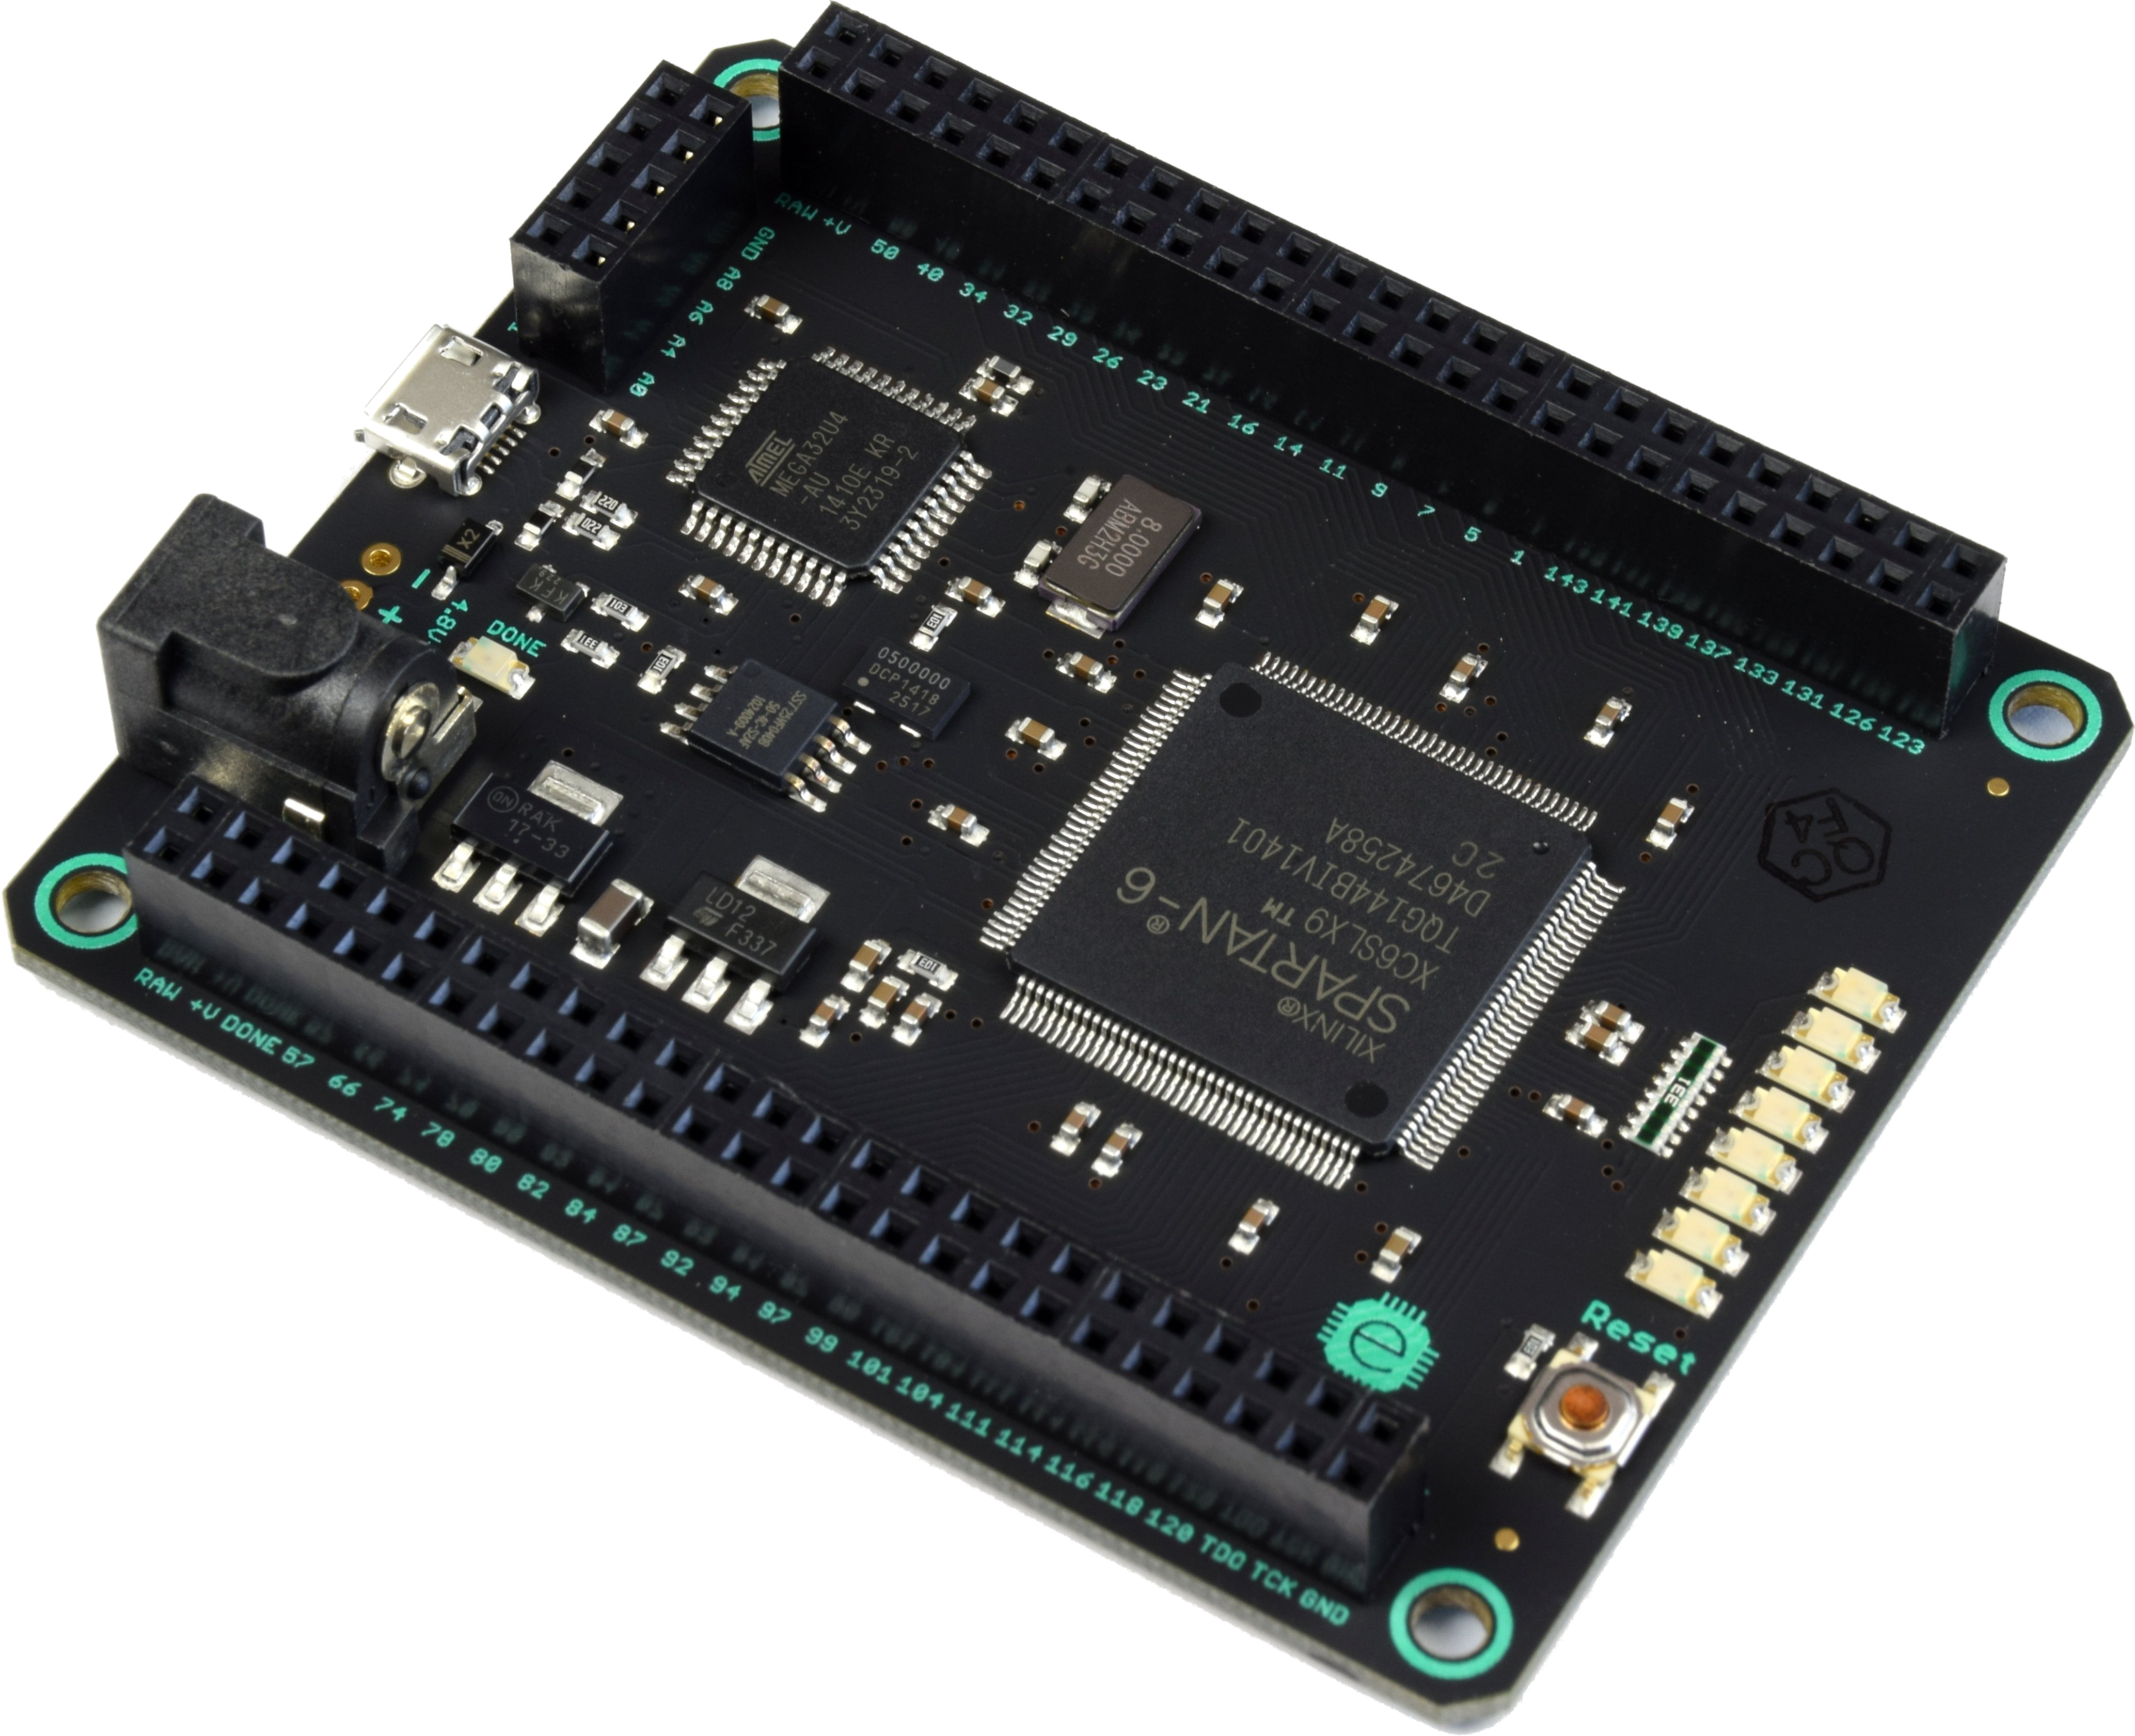
\includegraphics[width=\textwidth]{MojoIso.png}
%		\end{column}
%		\begin{column}{.55\textwidth}
%			\begin{itemize}
%				\only<1>{
%				\item FPGA Spartan 6 XC6SLX9 de Xilinx
%				\item 84 pines IO digitales
%				\item 8 entradas analógicas
%				\item 8 LEDs de propósito general
%				\item 1 pulsador de propósito general
%				\item ATmega32U4 para configurar la FPGA y leer los pines analógicos.
%				\item Memoria flash para almacenar la configuración de la FPGA.}
%				\item USB para programación y comunicación.
%				\only<2>{
%					\begin{itemize}
%						\item USB 2.0 Full-Speed de 12 Mbps
%						\item Implementado a través de controlador ATmega32U4
%						\item Interfaz FPGA-ATmega32U4 via SPI de 8 Mbps.
%					\end{itemize}
%			}
%			\end{itemize}
%		\end{column}
%	\end{columns}
%\end{frame}
%\begin{frame}{Estructura interna FPGA}
%	\centering
%	\begin{tikzpicture}[scale=.58]
%		\begin{scope}[transform shape,node distance=5,>=latex,thick]
%			\node[simple]	(cypress)		[]	 			{FIFO Esclava};
%			\node[simple]	(master)	[right=of cypress]	{Maestro Externo};
%			\node[simple,minimum size=70]	(leer)		[right=of master.north west,anchor=north west] {Leer FIFO};
%			\node[simple,minimum size=70]	(escribir)	[right=of master.south west,anchor=south west]	{Escribir FIFO};
%			\node[simple,node distance=8]	(fifo)		[right=of master]	{FIFO Interna (XLNX core generator)};
%			
%			\draw[<->]	([yshift=4*110/6]cypress.east) --node [above]{IFCLK} ([yshift=4*110/6]master.west);
%			\draw[<->]	([yshift=3*110/6]cypress.east) --node [above]{FD[15:0]} ([yshift=3*110/6]master.west);
%			\draw[<-]	([yshift=2*110/6]cypress.east) --node [above]{FIFOADR[1:0]} ([yshift=2*110/6]master.west);
%			\draw[->]	([yshift=1*110/6]cypress.east) --node [above]{EP2\_EMPTY} ([yshift=1*110/6]master.west);
%			\draw[->]	([yshift=0*110/6]cypress.east) --node [above]{EP8\_FULL} ([yshift=0*110/6]master.west);
%			\draw[<-]	([yshift=-1*110/6]cypress.east) --node [above]{SLOE} ([yshift=-1*110/6]master.west);
%			\draw[<-]	([yshift=-2*110/6]cypress.east) --node [above]{SLWR} ([yshift=-2*110/6]master.west);
%			\draw[<-]	([yshift=-3*110/6]cypress.east) --node [above]{SLRD} ([yshift=-3*110/6]master.west);
%			\draw[<-]	([yshift=-4*110/6]cypress.east) --node [above]{PKTEND} ([yshift=-4*110/6]master.west);
%			
%			\draw[<-] (leer) -- node[above]{SLWR} (master.east |- leer);
%			\draw[<-] ([yshift=-1*80/7]leer.east) -- node[above]{EMPTY}([yshift=-1*80/7]fifo.west |- leer);
%			\draw[->] ([yshift=1*80/7]leer.east) -- node[above]{RD\_EN}([yshift=1*80/7]fifo.west |- leer);
%			
%			\draw[<-] (escribir) -- node[above]{SLRD} (master.east |- escribir);
%			\draw[<-] ([yshift=-1*80/7]escribir.east) -- node[above]{FULL}([yshift=-1*80/7]fifo.west |- escribir);
%			\draw[->] ([yshift=1*80/7]escribir.east) -- node[above]{WR\_EN}([yshift=1*80/7]fifo.west |- escribir);			
%			
%			\draw[<-]	([yshift=1*110/6]fifo.west) --node [above]{DIN[15:0]} ([yshift=1*110/6]master.east);
%			\draw[->]	([yshift=0*110/6]fifo.west) --node [above]{DOUT[15:0]} ([yshift=0*110/6]master.east);
%			\draw[<-]	([yshift=-1*110/6]fifo.west) --node [above]{VALID} ([yshift=-1*110/6]master.east);
%			
%			\node[node distance=.4] (fpga) [above=of leer] {FPGA};
%		\end{scope}
%		\begin{scope}[on background layer]
%			\node[rectangle,rounded corners,dashed,fit=(master)(leer)(fpga)(fifo)(escribir),draw=black]{};
%		\end{scope}
%	\end{tikzpicture}
%\end{frame}
\begin{frame}{Interfaz - FPGA}
	\centering
	\begin{tikzpicture}[scale=.7]
		\begin{scope}[transform shape,node distance=4,>=latex,double distance=1.3]
			\node[simple](mef)[]{Maquina de Estados Finitos};
			\node[simple] (fifo) [left=of mef] {FIFO Esclava\\Controlador FX2LP};			
%				\node[simple,minimum size=80](clk)[right=of mef.north east,anchor=north west] {Fuente de reloj};
%				\draw[<-]([yshift=-1*80/3]mef.north east)--node[above]{Reloj}([yshift=-1*80/3]clk.north west);
%				\draw[<-]([yshift=-2*80/3]mef.north east)--node[above]{Reset}([yshift=-2*80/3]clk.north west);

			\node[simple,minimum width=85](interno)[right=of mef]{Sistema\\Implementado en FPGA};
			\draw[double,->]([yshift=5*220/8]mef.south east)--node[above](rec){Dato\_recibido[15:0]} ([yshift=5*220/8]interno.south west);
			\draw[double,<-]([yshift=4*220/8]mef.south east)--node[above](aEnv){Dato\_a\_enviar[15:0]}([yshift=4*220/8]interno.south west);
			\draw[<-]([yshift=3*220/8]mef.south east)--node[above](env){Enviar\_datos}([yshift=3*220/8]interno.south west);
			\draw[->]([yshift=2*220/8]mef.south east)--node[above](intrd){SLRD}([yshift=2*220/8]interno.south west);
			\draw[->]([yshift=1*220/8]mef.south east)--node[above](intwr){SLWR}([yshift=1*220/8]interno.south west);	
			\draw[<-]([yshift=-1*220/8]mef.north east)--node[above](clk){Reloj}([yshift=-1*220/8]interno.north west);
			\draw[<-]([yshift=-2*220/8]mef.north east)--node[above](rst){Reset}([yshift=-2*220/8]interno.north west);

			\draw[<->,thick] ([yshift=5*110/6]fifo.east) --node [above](ifclk){IFCLK} ([yshift=5*110/6]mef.west);
			\draw[<->,thick]	([yshift=4*110/6]fifo.east) --node [above](fd){FD[15:0]} ([yshift=4*110/6]mef.west);
			\draw[<-,thick]	([yshift=3*110/6]fifo.east) --node [above](fifoadr){FIFOADR[1:0]} ([yshift=3*110/6]mef.west);
			\draw[->,thick]	([yshift=2*110/6]fifo.east) --node [above](flaga){FLAGA} ([yshift=2*110/6]mef.west);
			\draw[->,thick]	([yshift=1*110/6]fifo.east) --node [above](flagb){FLAGB} ([yshift=1*110/6]mef.west);
			\draw[->,thick]	([yshift=0*110/6]fifo.east) --node [above](flagc){FLAGC} ([yshift=0*110/6]mef.west);
			\draw[->,thick]	([yshift=-1*110/6]fifo.east) --node [above](flagd){FLAGD} ([yshift=-1*110/6]mef.west);
			\draw[<-,thick]	([yshift=-2*110/6]fifo.east) --node [above](sloe){SLOE} ([yshift=-2*110/6]mef.west);
			\draw[<-,thick]	([yshift=-3*110/6]fifo.east) --node [above](slwr){SLWR} ([yshift=-3*110/6]mef.west);
			\draw[<-,thick]	([yshift=-4*110/6]fifo.east) --node [above](slrd){SLRD} ([yshift=-4*110/6]mef.west);
			\draw[<-,thick]	([yshift=-5*110/6]fifo.east) --node [above](pktend){PKTEND} ([yshift=-5*110/6]mef.west);
		\end{scope}
		\begin{scope}[]
			\node[draw=blue,dashed,rectangle,fit={(mef)(interno)},label=north:FPGA,rounded corners]{};
			\action<2>{\node[ultra thick,draw=blue,ellipse,fit=(fd)] {};}
			\action<3>{\node[ultra thick,draw=blue,ellipse,fit=(fifoadr)] {};}
			\action<4>{\node[ultra thick,draw=blue,ellipse,fit=(flaga)(flagb)] {};}
			\action<5>{\node[ultra thick,draw=blue,ellipse,fit=(sloe)] {};}
			\action<5>{\node[ultra thick,draw=blue,ellipse,fit=(slrd)] {};}
			\action<6>{\node[ultra thick,draw=blue,ellipse,fit=(slwr)] {};}
			\action<7>{\node[ultra thick,draw=blue,ellipse,fit=(pktend)] {};}
			\action<8>{\node[ultra thick,draw=blue,ellipse,fit=(clk)(rst)] {};}
			\action<9>{\node[ultra thick,draw=blue,ellipse,fit=(rec)] {};}
			\action<10>{\node[ultra thick,draw=blue,ellipse,fit=(aEnv)] {};}
			\action<11>{\node[ultra thick,draw=blue,ellipse,fit=(env)] {};}
			\action<12>{\node[ultra thick,draw=blue,ellipse,fit=(intrd)] {};}
			\action<13>{\node[ultra thick,draw=blue,ellipse,fit=(intwr)] {};}
		\end{scope}
	\end{tikzpicture}
\end{frame}

\begin{frame}{Operaciones en la FIFO}
	\framesubtitle{Escritura Asíncrona}
	\centering
		\begin{tikzpicture}[scale=.9]
			\begin{scope}[transform shape,node distance=1,text width=60]
				\setcounter{wavecount}{0}
				\newwave{FIFOADR[1]}
					\bit{0}{9}
				\newwave{FIFOADR[0]}
					\bit{0}{9}
				\newwave{FLAG\_Lleno}
					\only<-7>{
						\bit{1}{6}
						\bit{0}{3}}
					\only<8->{
						\bit{1}{4}
						\bit{0}{5}
					}
				\newwave{SLWR}
					\only<-7>{
						\bit{1}{3}
						\bit{0}{1}
						\bit{1}{1}
						\bit{0}{1}
						\bit{1}{1}
						\bit{0}{1}
						\bit{1}{1}
					}
					\only<8->{
						\bit{1}{3}
						\bit{0}{1}
						\bit{1}{1}
						\bit{0}{1}
						\bit{1}{1}
						\bit{0}{1}
						\bit{1}{1}
					}
				\newwave{PKTEND}
					\only<-7>{
						\bit{1}{9}
					}
					\only<8->{
						\bit{1}{3}
						\bit{0}{1}
						\bit{1}{5}
					}
				\newwave{FD[15:0]}
					\only<-7>{
					\bitvector{N-2}{3}
					\bitvector{N-1}{2}
					\bitvector{N}{2}
					\graybitvector{No leído}{2}	
					}
					\only<8->{
						\bitvector{N-20}{3}
						\bitvector{N-19}{2}
						\graybitvector{No leído}{4}
					}
				\action<2>{\draw[blue, ultra thick] (0.3,-0.6) ellipse (.6 and 1.2);}
				\action<3-5>{\draw[blue, ultra thick] (3.3,-3) ellipse (.5 and .6);}
				\action<4-5>{\draw[blue, ultra thick] (3.3,-5) ellipse (.5 and .6);}
				\action<5-6>{\draw[blue, ultra thick] (5.3,-3) ellipse (.5 and .6);}
				\action<5-6>{\draw[blue, ultra thick] (5.3,-5) ellipse (.5 and .6);}
				\action<6-7>{\draw[blue, ultra thick] (6.3,-2) ellipse (.5 and .6);}
				\action<7>{\draw[blue, ultra thick] (7.3,-3) ellipse (.5 and .6);}
				\action<7>{\draw[red, ultra thick] (8.3,-5) ellipse (1 and .6);}
				\action<9->{\draw[blue,ultra thick](3.3,-4)ellipse(.5 and .6);}
				\action<10->{\draw[blue,ultra thick](4.3,-2)ellipse(.5 and .6);}
				\action<10->{\draw[red,ultra thick](7.3,-5)ellipse(2 and .6);}
			\end{scope}
			\begin{scope}[on background layer]
				\foreach \x in {1,2,...,9}{
					\draw[dashed,black!20] (\x.3,0) -- (\x.3,\value{wavecount}+1);}
			\end{scope}
		\end{tikzpicture}
\end{frame}

\begin{frame}{Operaciones en la FIFO}
	\framesubtitle{Lectura Asíncrona}
	\centering
	\begin{tikzpicture}[scale=.9]
		\begin{scope}[transform shape,node distance=1,text width=60]
			\setcounter{wavecount}{0}
			\newwave{FIFOADR[1]}
				\bit{1}{9}
			\newwave{FIFOADR[0]}
				\bit{1}{9}
			\newwave{FLAG\_Vac\'io}
				\bit{1}{5}
				\bit{0}{4}
			\newwave{SLOE}
				\bit{1}{1}
				\bit{0}{7}
				\bit{1}{1}
			\newwave{SLRD}
				\bit{1}{2}
				\bit{0}{1}
				\bit{1}{1}
				\bit{0}{1}
				\bit{1}{1}
				\bit{0}{1}
				\bit{1}{2}
			\newwave{FD[15:0]}
				\bitvector{Z}{1}
				\bitvector{N-1}{2}
				\bitvector{N}{2}
				\graybitvector{No válido}{3}
				\bitvector{Z}{1}
			\action<2>{\draw[blue,ultra thick](.3,-.5)ellipse(0.5 and 1);}
			\action<3>{\draw[blue,ultra thick](1.3,-3)ellipse(0.5 and .6);}
			\action<3>{\draw[blue,ultra thick](0.8,-5)ellipse(0.5 and .6);}
			\action<4>{\draw[blue,ultra thick](2.3,-4.5)ellipse(0.6 and 1);}
			\action<5>{\draw[blue,ultra thick](3.3,-4.5)ellipse(0.5 and 1);}
			\action<6>{\draw[blue,ultra thick](5.3,-2)ellipse(0.5 and .6);}
			\action<6>{\draw[red,ultra thick](6.8,-5)ellipse(1 and .6);}
		\end{scope}
		\begin{scope}[on background layer]
			\foreach \x in {1,2,...,9}{
				\draw[dashed,black!20] (\x.3,0) -- (\x.3,\value{wavecount}+1);}
		\end{scope}
	\end{tikzpicture}
\end{frame}

\begin{frame}{Máquina de estados algorítmica de la interfaz}
	\centering
	\begin{tikzpicture}[ask/.style = {diamond,text width=70,draw=black,align=center,aspect=2},
	scale=.41]
		\begin{scope}[transform shape,node distance=(1 and 4),>=latex,]
			\node[moore,text width=110] (inicio) [label=above right:inicio]{FIFOADR=$''$ZZ$''$\\FDATA=$''$ZZ$''$\\d\_recibido=d\_recibido\\SLOE=$'1'$\\SLRD=$'1'$\\SLWR=$'1'$};
		
			\node[ask] (vacio1) [below=of inicio]{FLAG\_Vacío};
				\draw[->] (inicio.south) -| (vacio1);
		%			\node[moore,text width=100] (lecdir) [below=of vacio1,label=above right:dirección] {FIFOADR=entrada\\SLOE=$'0'$\\SLRD=$'1'$\\SLWR=$'1'$};
		%			\draw[o->](vacio1.east) -- ($(vacio1.east)+(1,0)$);
		
			\node[moore,text width=110] (lecoe) [right=of vacio1,label=above right:dir\_lect] {FIFOADR=$''11''$\\FDATA=$''$ZZ$''$\\d\_recibido=FD\\SLOE=$'0'$\\SLRD=$'1'$\\SLWR=$'1'$};
				\draw[->] (vacio1.east) -- ($(vacio1.east)!0.5!(lecoe.west)$);
				\draw[->]($(vacio1.east)!0.5!(lecoe.west)$) |- ($(lecoe.north)+(0,1)$) -- (lecoe.north);
		
			\node[moore,text width=110](lecrd)[below=of lecoe,label=above right:lectura]{FIFOADR=$''11''$\\FDATA=$''$ZZ$''$\\D\_recibido=FD\\SLOE=$'0'$\\SLRD=$'0'$\\SLWR=$'1'$};
				\draw[->](lecoe) -- (lecrd);
		
			\node[ask] (vacio2)[below=of lecrd]{FLAG\_Vacío};
				\draw[->](lecrd) -- (vacio2);
				
				\draw[->](vacio2.west) -| ($(lecoe.west)!.5!(vacio1.east)$);
				\draw[o->](vacio2.east) -- ++(1.5,0) |- ($(inicio.north)+(0,1)$);
				\draw[->] ($(inicio.north)+(0,1)$) -- (inicio.north);
		
			\node[ask](enviar1)[below=of vacio1]{Enviar\_datos};
				\draw[o->](vacio1.south) --(enviar1.north);
		
		
			\node[ask] (lleno1) [below=of enviar1]{FLAG\_Lleno};
				\draw[->](enviar1) -- (lleno1);
		
			\node[moore,text width=110](escdir)[below=of lleno1,label=above left:dir\_escr]{FIFOADR=$''00''$\\FDATA=d\_a\_enviar\\d\_recibido=d\_recibido\\SLOE=$'1'$\\SLRD=$'1'$\\SLWR=$'0'$};
				\draw[->](lleno1) -- ($(lleno1.south)!0.5!(escdir.north)$);
				\draw[->]($(lleno1.south)!0.5!(escdir.north)$) -- (escdir);
		
		
			\node[ask](vacio3)[left=of vacio1]{FLAG\_Vacío};
				\draw[->](escdir.south)--($(escdir.south)+(0,-.5)$) -| ($(vacio3.east)+(1,0)$) |- ($(vacio3.north)+(0,1)$)-|(vacio3.north);
		
			\node[ask](enviar2)[below=of vacio3]{Enviar\_datos};
				\draw[o->](vacio3) -- (enviar2);
		
				\draw[o->] (enviar1.west) -- ($(enviar1.west)+(-1,0)$);
				\draw[->] ($(enviar1.west)-(1,0)$) -- ($(inicio.north -| enviar1.west)+(-1,1)$);
				\draw[->] ($(inicio.north -| enviar1.west)+(-1,1)$)--($(inicio.north)+(0,1)$);
				\draw[->] ($(inicio.north)+(0,1)$) -- (inicio.north);
				\draw[o->](lleno1.west) -| ($(enviar1.west)-(1,0)$);
				\draw[->](vacio3.west) -- ($(vacio3.west)+(-1,0)$);
				\draw[->]($(vacio3.west)+(-1,0)$) |- ($(inicio.north -| enviar1.west)+(-1,1)$);
		
			\node[ask](lleno2)[below=of enviar2]{FLAG\_Lleno};
			\node[moore,text width=110](escwr)[below=of lleno2,label=above left:escribir]{FIFOADR=$''00''$\\FDATA=d\_a\_enviar\\d\_recibido=d\_recibido\\SLOE=$'1'$\\SLRD=$'1'$\\SLWR=$'1'$};
				\draw[->](lleno2) -- (escwr);
				\draw[o->](lleno2.west) -| ($(enviar2.west)+(-1,0)$);
				\draw[->](enviar2)--(lleno2);
				\draw[o->](enviar2)--($(enviar2.west)+(-1,0)$);
				\draw[->]($(enviar2.west)+(-1,0)$) -- ($(vacio3.west)+(-1,0)$);
				\draw[->](escwr) -- ($(escwr.south)+(0,-1)$) -| ($(escdir.east)+(1,0)$) |- ($(lleno1.south)!0.5!(escdir.north)$);
		\end{scope}
		\begin{scope}
			\action<2-3,7-8>{\node[ultra thick,draw=blue,ellipse,fit=(inicio)]{};}
			\action<6,11>{\node[ultra thick,draw=red,ellipse,fit=(inicio)]{};}
			\action<3,7>{\node[ultra thick,draw=red,ellipse,fit=(vacio1)]{};}
			\action<3,6>{\node[ultra thick,draw=red,ellipse,fit=(lecoe)]{};}
			\action<4>{\node[ultra thick,draw=blue,ellipse,fit=(lecoe)]{};}
			\action<5-6>{\node[ultra thick,draw=blue,ellipse,fit=(lecrd)]{};}
			\action<6>{\node[ultra thick,draw=red,ellipse,fit=(vacio2)]{};}
			\action<8>{\node[ultra thick,draw=red,ellipse,fit=(enviar1)]{};}
			\action<8>{\node[ultra thick,draw=red,ellipse,fit=(lleno1)]{};}
			\action<9-11,13>{\node[ultra thick,draw=blue,ellipse,fit=(escdir)]{};}
			\action<10>{\node[ultra thick,draw=red,ellipse,fit=(vacio3)(enviar2)(lleno2)]{};}
			\action<11>{\node[ultra thick,draw=red,ellipse,fit=(escwr)]{};}
			\action<12>{\node[ultra thick,draw=blue,ellipse,fit=(escwr)]{};}
		\end{scope}
	\end{tikzpicture}
\end{frame}

\begin{frame}{Verificación Funcional}
%	\only<1>{
%		\centering
%		\includegraphics[width=\textwidth]{tb_if_rd_mef}\\
%		\includegraphics[width=\textwidth]{tb_if_rd_end}
%	}
%	\only<2>{
		\framesubtitle{Operación de lectura}
		\centering
		\only<1>{\includegraphics[width=\textwidth]{mef_tb_lect00}}
		\only<2>{\includegraphics[width=\textwidth]{mef_tb_lect01}}
		\only<3>{\includegraphics[width=\textwidth]{mef_tb_lect02}}
		\only<4>{\includegraphics[width=\textwidth]{mef_tb_lect03}}
%	}
\end{frame}
\begin{frame}{Verificación Funcional}
	\framesubtitle{Operación de escritura}
	\centering
		\only<1>{\includegraphics[width=\textwidth]{mef_tb_escr00}}
		\only<2>{\includegraphics[width=\textwidth]{mef_tb_escr01}}
		\only<3>{\includegraphics[width=\textwidth]{mef_tb_escr02}}
		\only<4>{\includegraphics[width=\textwidth]{mef_tb_escr03}}

		\only<5>{\includegraphics[width=\textwidth]{mef_tb_full00}}
		\only<6>{\includegraphics[width=\textwidth]{mef_tb_full01}}
		\only<7>{\includegraphics[width=\textwidth]{mef_tb_full02}}
		\only<8>{\includegraphics[width=\textwidth]{mef_tb_full03}}
		\only<9>{\includegraphics[width=\textwidth]{mef_tb_full04}}
\end{frame}

%\begin{frame}{Implementación de la máquina de estados de la interfaz}
%	\scriptsize{
%		\only<1>{
%			\lstinputlisting[language=VHDL,firstline=20,lastline=28]{./codes/fx2lp_interface.vhd}
%			}
%		\only<2>{
%			\lstinputlisting[language=VHDL,firstline=29,lastline=48]{./codes/fx2lp_interface.vhd}
%		}
%		\only<3>{
%			\lstinputlisting[language=VHDL,firstline=50,lastline=67]{./codes/fx2lp_interface.vhd}
%		}
%		\only<4>{
%			\lstinputlisting[language=VHDL,firstline=69,lastline=76]{./codes/fx2lp_interface.vhd}
%		}
%		\only<5>{
%			\lstinputlisting[language=VHDL,firstline=78,lastline=92]{./codes/fx2lp_interface.vhd}
%		}
%		\only<6>{
%			\lstinputlisting[language=VHDL,firstline=94,lastline=113]{./codes/fx2lp_interface.vhd}
%		}
%		\only<7-8>{
%			\lstinputlisting[language=VHDL,firstline=115,lastline=118]{./codes/fx2lp_interface.vhd}}
%		\only<7>{
%			\begin{columns}[t]
%				\begin{column}{.5\textwidth}
%					\lstinputlisting[language=VHDL,firstline=119,lastline=134]{./codes/fx2lp_interface.vhd}
%				\end{column}				\begin{column}{.5\textwidth}
%					\lstinputlisting[language=VHDL,firstline=135,lastline=146]{./codes/fx2lp_interface.vhd}
%				\end{column}
%			\end{columns}
%		}
%		\only<8>{
%			\begin{columns}[t]
%				\begin{column}{.5\textwidth}
%					\lstinputlisting[language=VHDL,firstline=147,lastline=158]{./codes/fx2lp_interface.vhd}
%				\end{column}
%				\begin{column}{.5\textwidth}
%				\end{column}
%			\end{columns}
%			\lstinputlisting[language=VHDL,firstline=159,lastline=160]{./codes/fx2lp_interface.vhd}
%		}
%		\only<9>{
%			\lstinputlisting[language=VHDL,firstline=162,lastline=176]{./codes/fx2lp_interface.vhd}
%		}
%		\only<10>{
%			\lstinputlisting[language=VHDL,firstline=178,lastline=193]{./codes/fx2lp_interface.vhd}
%		}		
%		\only<11>{
%			\lstinputlisting[language=VHDL,firstline=195,lastline=206]{./codes/fx2lp_interface.vhd}
%		}
%	}
%\end{frame}
%\begin{frame}{Instanciación de la interfaz en el top}
%	\tiny{
%		\only<1>{
%			\lstinputlisting[language=VHDL,firstline=7,lastline=34]{./codes/fx2lp_interface_top.vhd}
%		}
%		\only<2>{
%			\lstinputlisting[language=VHDL,firstline=36,lastline=61]{./codes/fx2lp_interface_top.vhd}
%		}
%	}
%\end{frame}
%\begin{frame}{Maquinas de estado hacia la memoria FIFO interna}
%	\begin{columns}
%		\begin{column}{.5\textwidth}
%			\centering
%			\begin{tikzpicture}[scale=.53]
%				\begin{scope}[transform shape,node distance=1,>=latex]
%					\node[moore] (idle) {--idle:\\RE\_EN='0';};
%					\node[node distance=.6](aux0)[above=of idle]{};
%					\node[ask]	(pr1)	[below=of idle]{\tiny{SLWR='0'-$>$'1'}}
%						edge[<-] (idle);
%					\node[ask] (pr2) [below=of pr1]{\scriptsize{FIFO\_empty='1'}};
%					\node[node distance=.8](aux1)[left=of pr1]{};
%					\draw[->] (pr1) -- node[left] {Si} (pr2);
%					\draw[->] (pr1) -- node[above,near start]{No} (aux1.base);
%					\draw[->] (aux1.base) |- (aux0.base) -- (idle);
%					
%					\node[moore](rden)[below=of pr2]{--read enable:\\RD\_EN='1'};
%					\node[node distance=.8] (aux2) [left=of pr2] {};
%					\draw[->] (pr2) -- node[above,near start]{Si} (aux2.base);
%					\draw[->] (pr2) -- node[left,near start] {No} (rden);
%					\draw[->] (aux2.base) -- (aux1.base);
%					
%					\node[node distance=.8] (aux3) [below=of rden]{};
%					\draw[->] (rden) -- (aux3.base) -| (aux2.base); 
%				\end{scope}
%			\end{tikzpicture}
%		\end{column}
%		\begin{column}{.5\textwidth}
%			\centering
%			\begin{tikzpicture}[scale=.5]
%				\begin{scope}[transform shape,node distance=1,>=latex]
%					\node[moore] (idle) {--idle:\\WR\_EN='0';};
%					\node[node distance=.6](aux0)[above=of idle]{};
%					\node[ask]	(pr1)	[below=of idle]{\tiny{SLRD='0'-$>$'1'}}
%						edge[<-] (idle);
%					\node[ask] (pr2) [below=of pr1]{\scriptsize{FIFO\_FULL='1'}};
%					\node[node distance=.8](aux1)[left=of pr1]{};
%					\draw[->] (pr1) -- node[left] {Si} (pr2);
%					\draw[->] (pr1) -- node[above,near start]{No} (aux1.base);
%					\draw[->] (aux1.base) |- (aux0.base) -- (idle);
%					
%					\node[moore](rden)[below=of pr2]{--write enable:\\WR\_EN='1'};
%					\node[node distance=.8] (aux2) [left=of pr2] {};
%					\draw[->] (pr2) -- node[above,near start]{Si} (aux2.base);
%					\draw[->] (pr2) -- node[left,near start] {No} (rden);
%					\draw[->] (aux2.base) -- (aux1.base);
%					
%					\node[node distance=.8] (aux3) [below=of rden]{};
%					\draw[->] (rden) -- (aux3.base) -| (aux2.base); 
%				\end{scope}
%			\end{tikzpicture}
%		\end{column}
%	\end{columns}
%\end{frame}

		\subsection{Circuito de interconexión}
			\begin{frame}{Circuito de interconexión}
			\centering
			\rowcolors{2}{black!15}{white}
%	\begin{itemize}
%		\only<1>{
%			\item Versión 1\\
%			\centering
%			\includegraphics[width=.45\textwidth]{61v1anverso}
%			\includegraphics[width=.45\textwidth]{62v1reverso}
%		}			
		\only<1>{
%			\item Versión 2\\
			\includegraphics[width=.45\textwidth]{63v2anverso}
			\includegraphics[width=.45\textwidth]{64v2reverso}
		}
		\only<2>{
%			\item Versión 3\\
%			\centering
			\includegraphics[width=.45\textwidth]{65v3anverso}
			\includegraphics[width=.45\textwidth]{66v3reverso}
		}
		\only<3>{
			\begin{tabular}{lr|lr}
%				\hline
				\textbf{FX2LP} & \textbf{Spartan 6}&\textbf{FX2LP} & \textbf{Spartan 6} \\\hline
				FD15 & P50 &FD2 & P24\\
				FD14 & P51 &FD1 & P21\\
				FD13 & P40 &FD0 & P22\\
				FD12 & P41 &SLWR & P17\\
				FD11 & P34 &SLRD & P16\\
				FD10 & P35 &SLOE & P6\\
				FD9 & P32 &FLAGA & P12\\
				FD8 & P33 &FLAGB & P14\\
				FD7 & P29 &FLAGC & P15\\
				FD6 & P30 &FLAGD & P11\\
				FD5 & P26 &PKTEND & P10\\
				FD4 & P27 &FIFOADR1 & P9\\
				FD3 & P23 &FIFOADR0 & P8\\
%				\hline
			\end{tabular}
		}
%	\end{itemize}
\end{frame}
\begin{frame}{Sistema completo}
	\centering
	\includegraphics[width=.6\textwidth]{fisico}
\end{frame}

	\section{Evaluación y validación}
		\subsection{Desarrollo del sistema de pruebas}
			Una vez definidos los puertos y la MAE que se implementa, se está en condiciones de describirlo en un formato que sea sintetizable en una FPGA. El formato utilizado es el lenguaje VHDL (acrónimo del ingles {\it Very high speed Hardware Description Language}). A su vez, para sintetizar la descripción realizada, se recurre al programa ISE de Xilinx.

Considerando las señales descriptas en la Figura \ref{fpga:variables}, se obtendría un sistema que cumple con las especificaciones. Sin embargo, a fin de no dejar señales provistas por la interfaz al aire, se agregan todos FLAGS que brinda el controlador FX2LP en la entidad descripta. Además, se incorporan tres constantes para modificar a criterio del desarrollador las direcciones de entrada y salida, y el ancho del bus de datos, que puede ser de 8 o 16 bits. Por defecto, se utilizan las direcciones y ancho de bus. especificados en el Capitulo \ref{cap:cy}, es decir $''11''$ y $''00''$ como puertos de entrada y salida respectivamente y 16 bits de ancho de bus.

De lo anterior, podemos declarar la entidad que tiene los puertos detallados a continuación:

\begin{lstlisting}[language=VHDL,backgroundcolor=\color{gray!30}]
entity fx2lp_interfaz is
	generic(
		constant in_ep_addr:  std_logic_vector(1 downto 0) := "00";
		constant out_ep_addr: std_logic_vector(1 downto 0) := "11";
		constant port_width:  integer := 16
	);
	port(
		reloj: in std_logic;
		reset: in std_logic;
	-- desde y hacia la interfaz
	fdata:    inout std_logic_vector(port_width-1 downto 0);
	fifoaddr: out	std_logic_vector(1 downto 0);
	sloe: 	  out	std_logic;
	slrd:     out	std_logic;
	slwr:     out	std_logic;
	pktend:   out	std_logic;
	-- EP2 isoc in (hacia pc)
	-- EP8 bulk out (desde pc)
	flaga: in	std_logic;   -- EP2_full--->FLAG_Lleno
	flagb: in	std_logic;   -- EP8_empty-->FLAG_Vacio
	flagc: in	std_logic;   -- EP8_full--->sin uso
	flagd: in	std_logic;   -- EP2_empty-->sin uso
	-- desde y hacia el sistema
	enviar_dato: in  std_logic;
	d_recivido:  out std_logic_vector(port_width-1 downto 0);
	d_a_enviar:  in  std_logic_vector(port_width-1 downto 0)
);
end fx2lp_interfaz;
\end{lstlisting}

Luego, se describe el comportamiento de la máquina de estados que se implementa. El estilo elegido para la descripción cuenta con un registro que determina el estado próximo de la MAE a través de un proceso secuencial. El valor de dicho registro, es volcado a otro que indica el estado actual de la MAE, a través de los flancos del reloj, en una secuencia diferente. Las señales de salida son implementadas en forma concurrente, de manera externa a los procesos que comanda la MEA. Las señales de entrada se encuentran incorporadas en el proceso que determina el estado próximo.
La MEA es descripta a través del código que se muestra a continuación:

\begin{lstlisting}[language=VHDL,backgroundcolor=\color{gray!30}]
architecture Behavioral of fx2lp_interfaz is
	-- maquina de estados de la interfaz
	type estados_mea is
	(
		inicio,
		lec_direccion, lectura,
		esc_direccion, escritura
	);
	signal estado_actual, prox_estado: estados_mea := inicio;
begin
	--implementacion de la maquina de estados
	interfaz_mea: process(estado_actual, flag_lleno,
	 flag_vacio, enviar_dato)
	begin
		case estado_actual is
			when inicio =>
				if flag_vacio = '0' then
					prox_estado <= lectura;
				elsif enviar_dato = '1' then
					if flag_lleno = '0' then
						prox_estado <= escritura;
					else
						prox_estado <= inicio;
					end if;
				else
					prox_estado <= inicio;
				end if;

			when lec_direccion =>
				prox_estado <= lectura;

			when lectura =>
				if flag_vacio = '0' then
					prox_estado <= lec_direccion;
				else
					prox_estado <= inicio;
				end if;

			when esc_direccion =>
				prox_estado <= escritura;

			when escritura =>
				if enviar_dato = '1' then
					if flag_vacio = '1' and flag_lleno = '0' then
						prox_estado <= esc_direccion;
					else
						prox_estado <= inicio;
					end if;
				else
					prox_estado <= inicio;
				end if;

			when others =>
				prox_estado <= inicio;
		end case;
	end process interfaz_fsm;
end Behavioral;
\end{lstlisting}

En la descripción detallada anteriormente, los flags no coinciden con los puertos declarados. Para salvar esta inconsistencia, se declaran las señales utilizadas, {\it flag\_lleno} y {\it flag\_vacío} y se las asigna de forma concurrente a las señales {\it flaga} y {\it flagb}, respectivamente. Además, se coloca un inversor para hacer las señales activas en alto. Todo esto apunta a facilitar la lectura y el desarrollo de la descripción.

\begin{lstlisting}[language=VHDL,backgroundcolor=\color{gray!30}]
architecture Behavioral of fx2lp_interfaz is
	signal flag_vacio: std_logic;
	signal flag_lleno: std_logic;
begin
	flag_lleno  <= not flaga;
	flag_vacio <= not flagb;
end Behavioral;	
\end{lstlisting}

A su vez, también son necesarias señales que sirvan como conectores internos desde los puertos hacia los diferentes componentes que se describen.

\begin{lstlisting}[language=VHDL,backgroundcolor=\color{gray!30}]
architecture Behavioral of fx2lp_interfaz is
	signal slwr_int:  	 std_logic := '1';
	signal slrd_int:  	 std_logic := '1';
	signal sloe_int:  	 std_logic := '1';
	signal pktend_int:	 std_logic := '1';
	signal faddr_int:	 std_logic_vector(1 downto 0) := "ZZ";
	signal fdata_sal:	 std_logic_vector(port_width-1 downto 0);
	signal fdata_inent:	 std_logic_vector(port_width-1 downto 0);
	signal reloj_sitema: std_logic;
begin
	reloj_sistema <= reloj;
	slwr   <= slwr_int;
	slrd   <= slrd_int;
	sloe   <= sloe_int;
	faddr  <= faddr_int;
	pktend <= pktend_int;
	d_recibido <= fdata_ent;
	fdata_sal <= d_a_enviar;
	
end Behavioral
\end{lstlisting}

Con todas las señales definidas y asignadas, y la maquina de estados que se detalló anteriormente, se pueden asignar las señales de salida:

\begin{lstlisting}[language=VHDL,backgroundcolor=\color{gray!30}]
architecture Behavioral of fx2lp_interfaz is
	with estado_actual select
		faddr_int <=	out_ep_addr when lec_direccion | lectura,
						in_ep_addr  when esc_direccion | escritura,
						(others => 'Z') when others;
	
	slwr_int <=	'0' when prox_estado = esc_direccion else
				'1';
	
	slrd_int <= '0' when estado_actual = lec_direccion else
	'1';
	
	pktend_int <= ((not falg_vacio) or enviar_dato);
	
	with estado_actual select
	sloe_int <=	'0' when lectura | lec_direccion,
				'1' when others;
	
	with estado_actual select
		fdata <=	fdata_sal        when escritura | esc_direccion,
					(others => 'Z')  when others;
	
	with estado_actual select
		fdata_ent <=	fdata     when lectura | lec_direccion,
						fdata_ent  when others;
end Behavioral
\end{lstlisting}

Finalmente, resta el reloj que hace avanzar la MAE. A este reloj, se le acoplan dos temporizadores de habilitación. Esto se debe a que se espera que el sistema trabaje a 50 MHz. Sin embargo, para respetar los tiempos de establecimiento y ancho de pulso de las distintas señales\cite{Cypress2017}, cuando el próximo estado es esc\_dirección se deben esperar tres ciclos de reloj y en el caso de que el próximo estado sea escritura, lec\_direccion o lectura, se debe esperar dos ciclos de reloj.
Esto se implementa con dos contadores diferentes, los cuales habilitan o no el cambio de estado. Esto se detalla a continuación:

\begin{lstlisting}[language=VHDL,backgroundcolor=\color{gray!30}]
architecture Behavioral of fx2lp_interfaz is
	signal cont3:	 natural range 0 to 4 := 0;
	signal cont2:	 natural range 0 to 3 := 0;
	signal disparo3: std_logic := '0';
	signal disparo2: std_logic := '0';
begin
	contador3: process(reloj_sistema, reset, disparo3)
	begin
		if reset = '0' then
			cont3 <= 0;
		elsif rising_edge(reloj_sistema) then
			if cont3 > 0 then
				cont3 <= cont3 - 1;
			elsif disparo3 = '1' then
				cont3 <= 4;
			end if;
		end if;
	end process contador3;

	disparo3 <= '1' when (prox_estado = esc_direccion) else '0';
	
	counter2: process(reloj_sistema, reset, disparo2)
	begin
		if reset = '0' then
			cont2 <= 0;
		elsif rising_edge(reloj_sistema)then
			if cont2 > 0 then
				cont2 <= count2 - 1;
			elsif disparo2 = '1' then
				cont2 <= 3;
			end if;
		end if;
	end process contador2;
	
	with prox_estado select
	disparo2 <=	'1' when lec_direccion | lectura | esc_direccion,
				'0' when others;

	reloj_mea: process (reloj_sistema, reset)
	begin
		if reset = '0' then
				estado_actual <= idle;
		elsif rising_edge(reloj_sistema) then
			if cont2 = 0 and cont3 = 0 then
				estado_actual <= prox_estado;
			end if;
		end if;
	end process reloj_mea;
end Behavioral
\end{lstlisting}

El código completo se puede encontrar en el Anexo \ref{ap:vhdl}

%			\begin{frame}{Depuración de la interfaz en VHDL}
	\begin{itemize}
		\item Se utilizó un registro para elaborar un eco de a dos bytes. Permitió corroborar el correcto funcionamiento de la lectura y escritura de las memorias FIFO de la interfaz de Cypress.
		\item Se utilizó una memoria FIFO generada con el software ``Core Generator'' de Xilinx para lograr un correcto funcionamiento de las señales de la interfaz escrita en VHDL.
		\item Además, se utilizó un PLL como generador de reloj, ya que si bien se pensaba hacer sincrónico, por errores de diseño esto no fue posible.
	\end{itemize}
\end{frame}

%		\subsection{Depuración de firmware del puente}
%			\begin{frame}{Debug Cypress}
	\begin{itemize}
		\item Se utilizó el framework provisto por Cypress para ser compilado con SDCC. No dió los frutos esperados.
		\item Se utilizó el framework provisto por Cypress para ser compilado con C51 de Keil. No funcionó en primera instancia.
		\item Se programó el puerto UART del 8051 para rastrear el error.
		\item Se logró que el framework trabaje adecuadamente solo con el puerto UART funcionando.
		\item Se utilizaron los LEDs indicadores para corroborar el llenado y vaciamiento de los extremos.
		\item Se aprovecharon los botones indicadores para corroborar el correcto funcionamiento de los extremos.
	\end{itemize}
\end{frame}

%		\subsection{Biblioteca de PC}
%				libusb es una biblioteca de código abierto, muy bien documentada, escrita en C, que brinda acceso genérico a dispositivos USB. Las características de diseño que persigue el equipo de desarrollo que mantiene la biblioteca es que sea multiplataforma, modo usuario y agnótico de versión.\\
	
	En el sitio web disponible %TODO cita a libusb.info
	se explica lo que significa cada uno de estos conceptos:
	
	\begin{itemize}
		\item{Multiplataforma:} Se apunta a que cualquier software que contenga esta biblioteca pueda ser compilado y ejecutado en la mayo cantidad de plataformas posibles, dotando al software de portabilidad, es decir, ala biblioteca puede ser ejecutada en Windows, Linux, OS X, Android y otras plataformas sin necesidad de realizar cambios en el código.
		\item{Modo usuario:} No se requiere acceso privilegiado de ningún tipo para poder ejecutar programas escritos con esta biblioteca.
		\item{Agnótisco de versión:} Sin importar la versión de la norma USB que se utilice, el programa se podrá comunicar siempre con el dispositivo USB que se requiera.
	\end{itemize}
	
	Otra ventaja que posee la biblioteca libusb es que, al ser de código abierto, posee una gran comunidad que contribuye al crecimiento del proyecto, como así también otros proyectos que utilizan esta biblioteca. Así, existe una gran variedad de ejemplos que facilitan el aprendizaje en su utilización y adaptaciones para diferentes lenguajes de programación, que se adapte a los conocimientos previos de la persona que desarrolla programas.
		\subsection{Desarrollo de un programa de pruebas}
			\begin{frame}{Esquemas de prueba}
	\centering
	\begin{tikzpicture}[scale=.8,>=latex]
		\begin{scope}[transform shape,node distance=1]
			\node[mealy]	(init)	[]{Inicializacion;};
			\node[mealy] (snd) [below=of init]{Enviar Datos;}
				edge[<-] (init);
			\node[mealy] (rcv) [below=of snd]{Recibir Datos;}
				edge[<-] (snd);
			\draw[<-] (rcv) to [in=0,loop,looseness=5] (rcv);
			\node[mealy](cmpr)[below=of rcv]{Comparar;\\Guardar\\en archivo;}
				edge[<-] (rcv);
			\draw[->] (cmpr) to [in=180,out=180,loop,looseness=1] (snd);
		\end{scope}
	\end{tikzpicture}
\end{frame}

\begin{frame}{Sistema en funcionamiento}
	\centering
	\includegraphics[width=\textwidth]{sistema2}
\end{frame}

	\section{Resultados y conclusiones}
		\subsection{Pruebas y resultados}
			\begin{frame}{Resultados de la prueba de comunicación}
	\begin{itemize}
		\item El sistema envió y recibió paquetes durante 24 horas, logrando la correcta transmisión y recepción de 388.191.289 paquetes de 128 bytes cada uno.
		\item El sistema desarrollado estableció una comunicación USB de alta velocidad.
		\item La tasa de transferencia de datos es de 12,4 Mbps.
		\item No hubo perdida ni errores en los datos transmitidos.
		\item La tasa efectiva de transmisión de datos útiles fue de 9,12 Mbps.
	\end{itemize}
\end{frame}
		\subsection{Conclusiones}
			\begin{frame}{Concluiones}
	\begin{itemize}
		\item Se elaboró un sistema de comunicación USB que permite conectar una FPGA con una PC, mediante una interfaz comercial.
		\item El sistema elaborado permite leer y escribir datos en forma robusta, es decir, sin perder datos.
		\item El sistema elaborado alcanzó una tasa de transferencia de 12 Mbps.
		\item Se aprendió sobre las técnicas y herramientas que permiten desarrollar y depurar sistemas en VHDL, C para microcontoladores y C para computadoras.
		\item Se desarrollaron competencias sobre las formas de prueba y validación de los sistemas implementados y sus componentes.
	\end{itemize}
\end{frame}

		\subsection{Trabajo futuro}
			\begin{frame}{Lo que falta...}
	\begin{itemize}
		\item Realizar una prueba de máxima transferencia de datos.
		\item Elaborar la documentación necesaria para que la interfaz de comunicación pueda ser utilizada por otros desarrolladores
	\end{itemize}
\end{frame}
\begin{frame}{Consultas}
	Consultas y sugerencias.
\end{frame}
\begin{frame}[c]
	\centering
	\alert {Muchas gracias.}
\end{frame}
			
%			\begin{frame}{Material Adicional}
%			\end{frame}
%			\tiny{
%			\lstinputlisting[language=VHDL]{codes/fx2lp_interface.vhd}
%			\lstinputlisting[language=VHDL]{codes/fx2lp_interface_top.vhd}
%			\lstinputlisting[language=VHDL]{codes/fx2lp_interface_top.ucf}
%			\lstinputlisting[language=VHDL]{codes/interface_test_bench.vhd}	
%			\includegraphics[width=\textwidth]{tb_top_sys_init}\\
%			\includegraphics[width=\textwidth]{tb_top_rd_init}\\
%			\includegraphics[width=\textwidth]{tb_top_rd_end}\\
%			\includegraphics[width=\textwidth]{tb_top_rd_end_det}\\
%			\includegraphics[width=\textwidth]{tb_top_wr_init}\\
%			\includegraphics[width=\textwidth]{tb_top_wr_end}\\
%			\lstinputlisting[language=C]{./codes/bridge.c}
%			\lstinputlisting[language=C++]{./codes/tfUSBCheck.cpp}
%			\lstinputlisting[language=C++]{./codes/tfUSBCheck.h}
%			}
\end{document}